\chapter{系统前端及初始化}
\label{chap:3}
本章主要研究系统的前端和初始化相关内容,其中前端主要包括视觉信息预处理和IMU预积分,视觉信息预处理包括特征提取和跟踪,异常点剔除。初始化主要包括多视图几何基础,visual初始化,以及Visual-IMU联合初始化。
\section{视觉信息预处理}
在视觉SLAM中,前端也称为视觉里程计(Visual Odometer,VO)\upcite{高翔2017视觉}。VO的实现方法有很多,包括特征点法,直接法和光流法。特征点法需要提取特征点,这包括提取关键点和计算描述子,然后进行特征匹配;直接法是从光流法继承而来的,不需特征提取及匹配;光流法不进行特征点匹配,取而代之的是利用光流跟踪特征点。表\ref{tab:3.1}列出了三种方法的优缺点。综合考虑,本文选用光流法作为视觉前端算法。
\begin{table}[h]\setlength{\abovecaptionskip}{6pt} 
	\zihao{5}  
	\centering
	\caption{特征点法、直接法和光流法对比} \label{tab:3.1}
	\begin{tabular}{m{0.1\textwidth}<{\centering} m{0.22\textwidth}<{\centering}  m{0.24\textwidth}<{\centering} m{0.26\textwidth}<{\centering} }%
		\toprule
		优缺点	   &   特征点法   &  	直接法	  &   光流法 \\
		\midrule
		优点	   &(1)对比直接法和光流法,鲁棒性高;(2)不受照影响。&(1)不需要特征点提取和匹配,计算量小;(2)可以在无纹理或者重复纹理场景下工作;(3)可以构建半密集或密集地图。 &(1)不需要计算描述子和匹配特征,计算量小;(2)可以在无纹理或者重复纹理场景下工作;(3)容易移植到嵌入式系统中,方便IMU进行融合;(4)可以构建半密集或者密集的地图。 \\
		缺点 &(1)在无纹理或者重复纹理场景下无法工作;(2)计算量大,不能保证实时性;(3)仅用CPU无法构建半稠密或稠密地图。  &(1)基于灰度不变假设,对光照变化敏感;(2)单个像素没有区分度,需要计算像素块;(3)图像是非凸的,容易产生局部极值。&(1)基于灰度不变假设,对光照变化敏感;\\	
		\bottomrule
	\end{tabular}
\end{table} 

\subsection{关键点和关键帧}
关键点也可以称为角点,它与特征点的区别是它没有描述子。常用的角点检测算法有Harris角点\upcite{harris1988combined}和FAST角点\upcite{rosten2006machine}。相比于Harris角点,FAST角点检测速度更快,因为FAST角点不需要计算像素的梯度,仅仅通过比较周围像素的亮度来确定是否为角点。如图\ref{fig3_1},它的算法流程如下:

(1)选取图像中的一个像素 $p$ ,设其亮度为 $I_p $ ;

(2)设定一个合适的亮度阈值 $T$ (例如设为 $I_p $ 的 20\%  );

(3)以像素  $p$  为圆心,画半径为3像素的圆,并选取圆上的所有像素(16个);

(4)如果在这16个像素点中,有连续 $N $  个点的亮度都大于$I_p+T $ 或者小于 $I_p-T $,那么像素 $p $ 就是角点。通常$N $  取12,9和11,分别称为FAST-12,FAST-9和FAST-11;

(5)对图像中的每一个像素执行以上步骤,提取所有的角点。
\begin{figure}[h]\setlength{\belowcaptionskip}{-12pt}
	\centering
	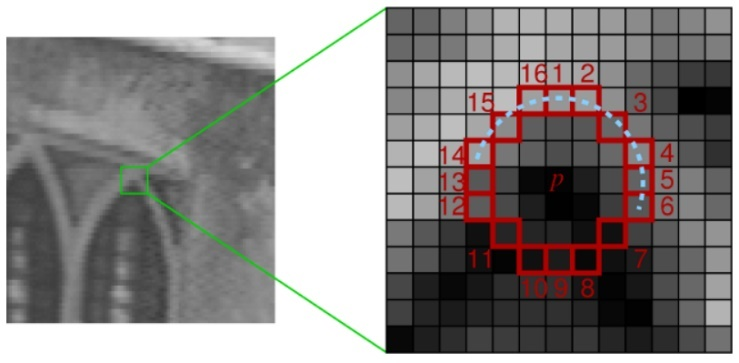
\includegraphics[width=0.5\textwidth]{figures/chapter3/fig3_1}
	\caption{FAST角点}\label{fig3_1}
\end{figure}

针对FAST-12算法,为了提高检测效率,可以添加一个预判别的操作,用来排除掉大部分不是角点的像素点。方法为:直接检测像素 $p$ 周围第1,5,9和13个像素点的亮度。当这四个像素中有三个像素的亮度同时大于$I_p+T $ 或者小于$I_p-T $ 时,该像素才有可能是角点,才会继续利用FAST-12进行角点检测,否则直接排除该像素。这样的预判别操作大幅度提升了角点检测的速度。

增加预判操作确实可以大大提高算法效率,但是到此为止算法还存在一个缺点,检测出来的很多相邻的角点挤在一起。为了消除这种邻近位置有多个角点重合的情况,需要进行非大极值抑制(Non-Maximal Suppression,NMS)\upcite{blaschko2011branch}。方法如下:

(1)计算每一个检测到的角点的响应值(score function) $V$,这里$V$ 定义为角点点 $p$ 和它邻域16个像素点的绝对差值之和,即,
\[
\setlength{\abovedisplayskip}{6pt}
\setlength{\belowdisplayskip}{6pt}
V = \Sigma_{x \in S} |I_{p\rightarrow x} - I_p|
\] 
其中 $S$ 表示16的邻域像素点的集合。

(2)考虑两个相邻的角点,并比较它们的 $V$ 值,并删除 $V$ 值较小的角点。
图\ref{fig3_2}展示了FAST角点提取。其中,(a)是原始图像,(b)是不加NMS 的FAST角点提取,(c)是加入NMS的FAST角点提取。
\begin{figure}[h]\setlength{\belowcaptionskip}{-12pt}
	\centering
	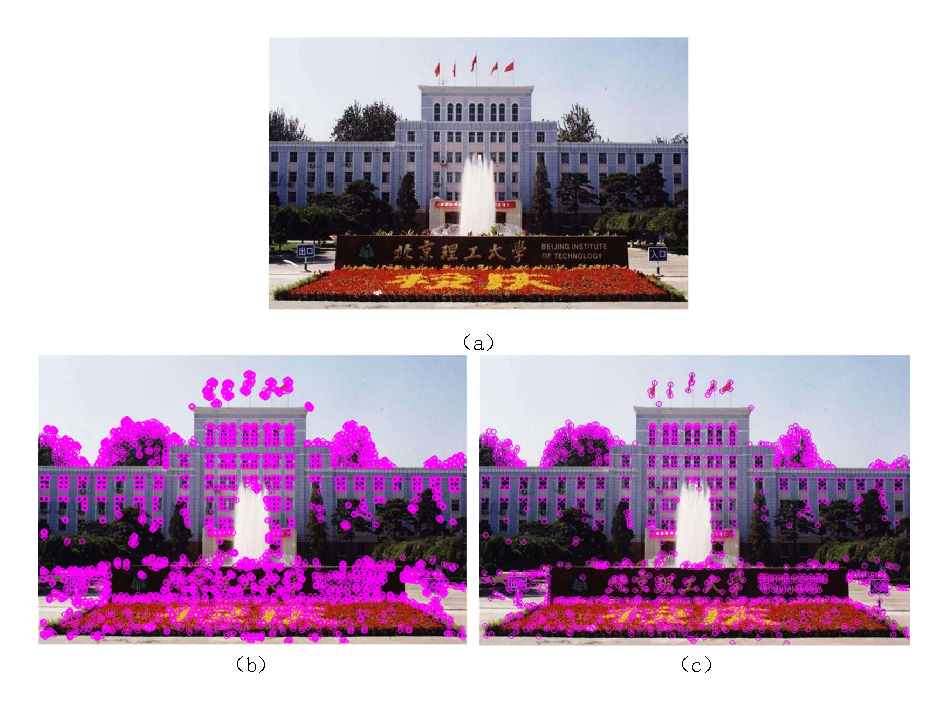
\includegraphics[width=0.9\textwidth]{figures/chapter3/fig3_2}
	\caption{(a)原始图像;(b)不加NMS 的FAST角点提取;(c)加入NMS的FAST角点提取。}\label{fig3_2}
\end{figure}

考虑到系统的实时性,不会对所有的图像都进行关键点提取,而是引入关键帧机制,即只对关键帧提取关键点,非关键帧则直接忽略。本文依据两个标准来选择关键帧。第一,两个关键帧之间要有足够的视差。当跟踪到的特征的平均视差介于当前帧和最近的关键帧视差之间,则将当前帧视为新的关键帧。第二,每张图像跟踪到的关键点要大于某一阈值,否则,将该帧视为关键帧。这样做是为了防止图像关键点完全跟丢,导致系统崩溃。
\subsection{特征跟踪}
关键点检测出来后就需要对其进行跟踪,本文采用光流跟踪关键点。光流是用来描述像素在图像中随着时间运动的方法,如图\ref{fig3_3}所示。跟踪部分像素的运动称为稀疏光流,跟踪所有像素的运动称为稠密光流。在SLAM中通常用LK(Lucas-Kanade)光流\upcite{bouguet2001pyramidal}来跟踪关键点的位置。
\begin{figure}[h]\setlength{\belowcaptionskip}{-12pt}
	\centering
	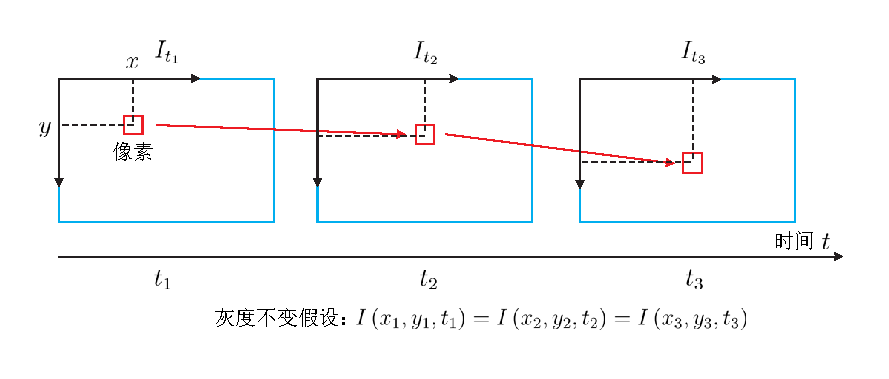
\includegraphics[width=0.8\textwidth]{figures/chapter3/fig3_3}
	\caption{LK光流法示意图}\label{fig3_3}
\end{figure}

在LK光流中,相机是运动的,也就是说相机的图像随着时间的变化而变化。所以,图像和时间之间存在一个映射关系:$\bm{I}(t) $ 。那么,在 $t$ 时刻,图像中 $(x,y)$ 处的像素的灰度可以记作:$ \boldsymbol{I}(x, y, t) $ 。这样,图像就是关于位置和时间的函数,该函数的值域就是图像的灰度。假设三维空间中的一个点 $p$ 在 $t$  时刻时的像素坐标为 $(x,y)$ 。随着时间的变化,$p$ 的像素坐标将发生变化。要估计出每一时刻该点的像素坐标。
首先,需要提出一个基本的假设:灰度不变假设。即三维空间中的点在每张图像中的像素灰度值是固定不变的。例如,在 $t+\mathrm{d} t $ 时刻点  $p$ 的像素坐标为 $(x+\mathrm{d} x, y+\mathrm{d} y) $ ,则,
\begin{equation}
\label{eqn:3.1}
\boldsymbol{I}(x+\mathrm{d} x, y+\mathrm{d} y, t+\mathrm{d} t)=\boldsymbol{I}(x, y, t)
\end{equation}
对式(\ref{eqn:3.1})左边用泰勒公式展开并保留一阶项,得,
\begin{equation}
\label{eqn:3.2}
\boldsymbol{I}(x+\mathrm{d} x, y+\mathrm{d} y, t+\mathrm{d} t) \approx \boldsymbol{I}(x, y, t)+\frac{\partial \boldsymbol{I}}{\partial x} \mathrm{d} x+\frac{\partial \boldsymbol{I}}{\partial y} \mathrm{d} y+\frac{\partial \boldsymbol{I}}{\partial t} \mathrm{d} t
\end{equation}
由式(\ref{eqn:3.1})和(\ref{eqn:3.2})得,
\begin{equation}
\label{eqn:3.3}
\frac{\partial \boldsymbol{I}}{\partial x} \mathrm{d} x+\frac{\partial \boldsymbol{I}}{\partial y} \mathrm{d} y+\frac{\partial \boldsymbol{I}}{\partial t} \mathrm{d} t=0
\end{equation}
\begin{equation}
\label{eqn:3.4}
\frac{\partial \boldsymbol{I}}{\partial x} \frac{\mathrm{d} x}{\mathrm{d} t}+\frac{\partial \boldsymbol{I}}{\partial y} \frac{\mathrm{d} y}{\mathrm{d} t}=-\frac{\partial \boldsymbol{I}}{\partial t}
\end{equation}
其中,$\mathrm{d} x / \mathrm{d} t $ 和 $\mathrm{d} y / \mathrm{d} t $ 分别表示像素在 $x$ 轴方向和 $y$ 轴方向上的速度分量,将其分别记为 $u, v $ 。$\partial \boldsymbol{I} / \partial x $ 和 $\partial \boldsymbol{I} / \partial y $ 表示 $x$ 轴方向和 $y$轴方向上的像素梯度,分别记为 $\boldsymbol{I}_{x}, \boldsymbol{I}_{y} $ 。$\partial \boldsymbol{I} / \partial t $ 表示图像灰度随时间的变化量,记为$\boldsymbol{I}_{t} $ 。这样可以将式(\ref{eqn:3.4})写成如下矩阵形式,
\begin{equation}
\label{eqn:3.5}
\left[ \begin{array}{ll}{\boldsymbol{I}_{x}} & {\boldsymbol{I}_{y}}\end{array}\right] \left[ \begin{array}{l}{u} \\ {v}\end{array}\right]=-\boldsymbol{I}_{t}
\end{equation}

假设在图像中的某一个 $w \times w $ 大小的窗口内所有的像素(共有 $w^2 $ 个)具有相同的运动,那么可以得到 $w^2 $ 个方程,
\begin{equation}
\label{eqn:3.6}
\left[ \begin{array}{cc}{\boldsymbol{I}_{x}} & {\boldsymbol{I}_{y}}\end{array}\right]_{k} \left[ \begin{array}{c}{u} \\ {v}\end{array}\right]=-\boldsymbol{I}_{t k}, \quad k=1, \ldots, w^{2}
\end{equation}
记,
\begin{equation}
\label{eqn:3.7}
A=\left[ \begin{array}{c}{\left[\boldsymbol{I}_{x}, \boldsymbol{I}_{y}\right]_{1}} \\ {\vdots} \\ {\left[\boldsymbol{I}_{x}, \boldsymbol{I}_{y}\right]_{k}}\end{array}\right], \boldsymbol{b}=\left[ \begin{array}{c}{\boldsymbol{I}_{t 1}} \\ {\vdots} \\ {\boldsymbol{I}_{t k}}\end{array}\right]
\end{equation}
所以,式(\ref{eqn:3.6})可以写为,
\begin{equation}
\label{eqn:3.8}
\boldsymbol{A} \left[ \begin{array}{l}{u} \\ {v}\end{array}\right]=-\boldsymbol{b}
\end{equation}
使用最小二乘法求解式(3.8),
\begin{equation}
\label{eqn:3.9}
\left[ \begin{array}{c}{u} \\ {v}\end{array}\right]^{*}=-\left(\boldsymbol{A}^{T} \boldsymbol{A}\right)^{-1} \boldsymbol{A}^{T} \boldsymbol{b}
\end{equation}

这样就可以计算处像素的运动速度 $u,v$ ,从而计算出像素在图像中的位置。也就实现了使用LK光流来跟踪角点的目的。
图\ref{fig3_4}是光流跟踪FAST角点示意图。其中,左图(a)中的点是检测到的FAST角点,右图(b)是相机向左平移一段距离拍摄的图像,蓝线是LK光流跟踪角点的轨迹。
\begin{figure}[h]\setlength{\belowcaptionskip}{-12pt}
	\centering
	\subfigure[FAST角点]{
		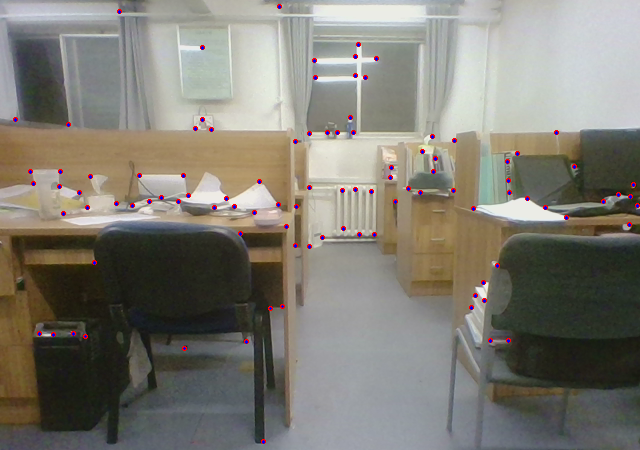
\includegraphics[width=0.4\textwidth]{figures/chapter3/LK1}}
	\subfigure[LK跟踪]{
		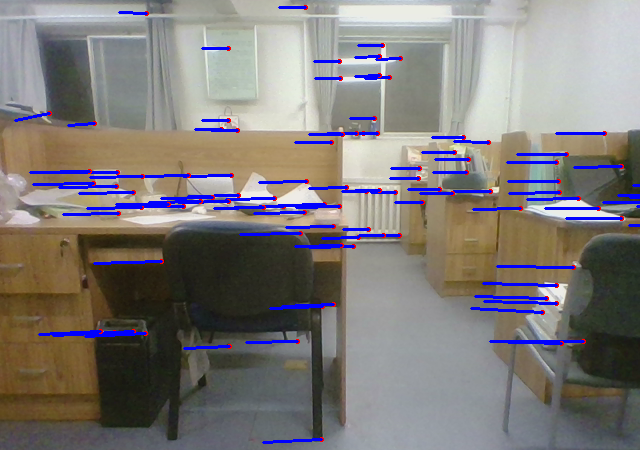
\includegraphics[width=0.4\textwidth]{figures/chapter3/LK2}}
	\caption{光流跟踪FAST角点}\label{fig3_4}
\end{figure}
\subsection{异常点剔除}
在视觉SLAM中,不管是特征点匹配还是光流跟踪都会出现误匹配或误跟踪的情况,那些匹配正确或者跟踪正确的点称为“局内点(inlier)”,而匹配错误或者跟踪错误的点称为“局外点(outlier)” 或者“异常点”。这些“异常点”会影响SLAM的定位精度,因此需要对其进行剔除。

在视觉SLAM中剔除“outlier”常用的方法是RANSAC(Random Sample Consensus),该算法是Fischler和Bolles等人于1981年最先提出的\upcite{fischler1981random2}。它可以得到有效的数据,即“局内点”,剔除无用数据,即“局外点”。在实践中,“异常点”通常是由于测量错误、假设错误和计算错误等原因造成,他们通常与正确数据“相距”很远。

该算法假设:

(1)样本数据集包含“局内点”和“局外点”;

(2)“局外点”不满足计算假设的数学模型;

(3)“局内点”满足某一数学模型,并可以计算其参数;

(4)其余数据是噪声数据。

该算法步骤如下:

(1)从样本数据集 $S$ 中随机选取一小组点集 $s$ (共有 $n$ 个),假设 $s$  的所有点为“局内点”,通过该点集得到一个数学模型 $F$ ;

(2)用该数学模型 $F$ 去测试 $S$ 中除 $s$ 外的其他点,并假设满足该数学模型的点为“局内点”;

(3)如果被假设为“局内点”的数量 $n$ 大于设定的阈值 $T$ ,那么就认为数学模型 $F$ 是合理的;

(4)用所有假设的“局内点”重新估计数学模型 ;

(5)如果迭代次数大于等于 $k$ ,则停止,否则重复上述步骤。

关键在于如何确定 $k$ 值。假设在样本数据集中“局内点”的概率是 $w $ ,则,
\begin{equation}
\label{eqn:3.10}
w = \frac{n_{inliers}}{n_{inliers} + n_{outliers}}
\end{equation}

最少需要假设 $n$ 个“局内点”确定模型 $F$ ,$n$ 视具体问题而定。$n$ 个假设的“局内点”都是实际的“局内点”的概率为 $w^n$ ,$n$ 个假设的“局内点”中至少有一个是实际的“局外点”的概率为 $1-w^n $ 。$k$ 次随机选取的点集 $s$ 中没有一次全部是“局内点”的概率是 $(1-w^n)^k $ ,用  $P$ 表示 $k$ 次随机选取的点集 $s$  中全部都是“局内点”的概率, $P$ 也表示取到正确解的概率或者置信度,则,
\begin{equation}
\label{eqn:3.11}
\setlength{\abovedisplayskip}{6pt}
\setlength{\belowdisplayskip}{6pt}
P=1-(1-w^n)^k
\end{equation}
“局内点”的概率 $w$  是一个先验值,可以根据先验假设一个初值。此时,可以计算出迭代次数 $k$  ,
\begin{equation}
\label{eqn:3.12}
k = \frac{log(1-P)}{log(1-w^n)}
\end{equation}
以上是“异常点”剔除的通用步骤,下面研究RANSAC是如何剔除关键点的。
以计算基本矩阵来剔除“异常点”为例,则上面研究的数学模型 $F$ 为基本矩阵。使用8点法计算 $F $ ,则 $n=8$ 。图\ref{fig3_5}展示了使用基本矩阵剔除异常点的步骤。
\begin{figure}[h]\setlength{\belowcaptionskip}{-12pt}
	\centering
	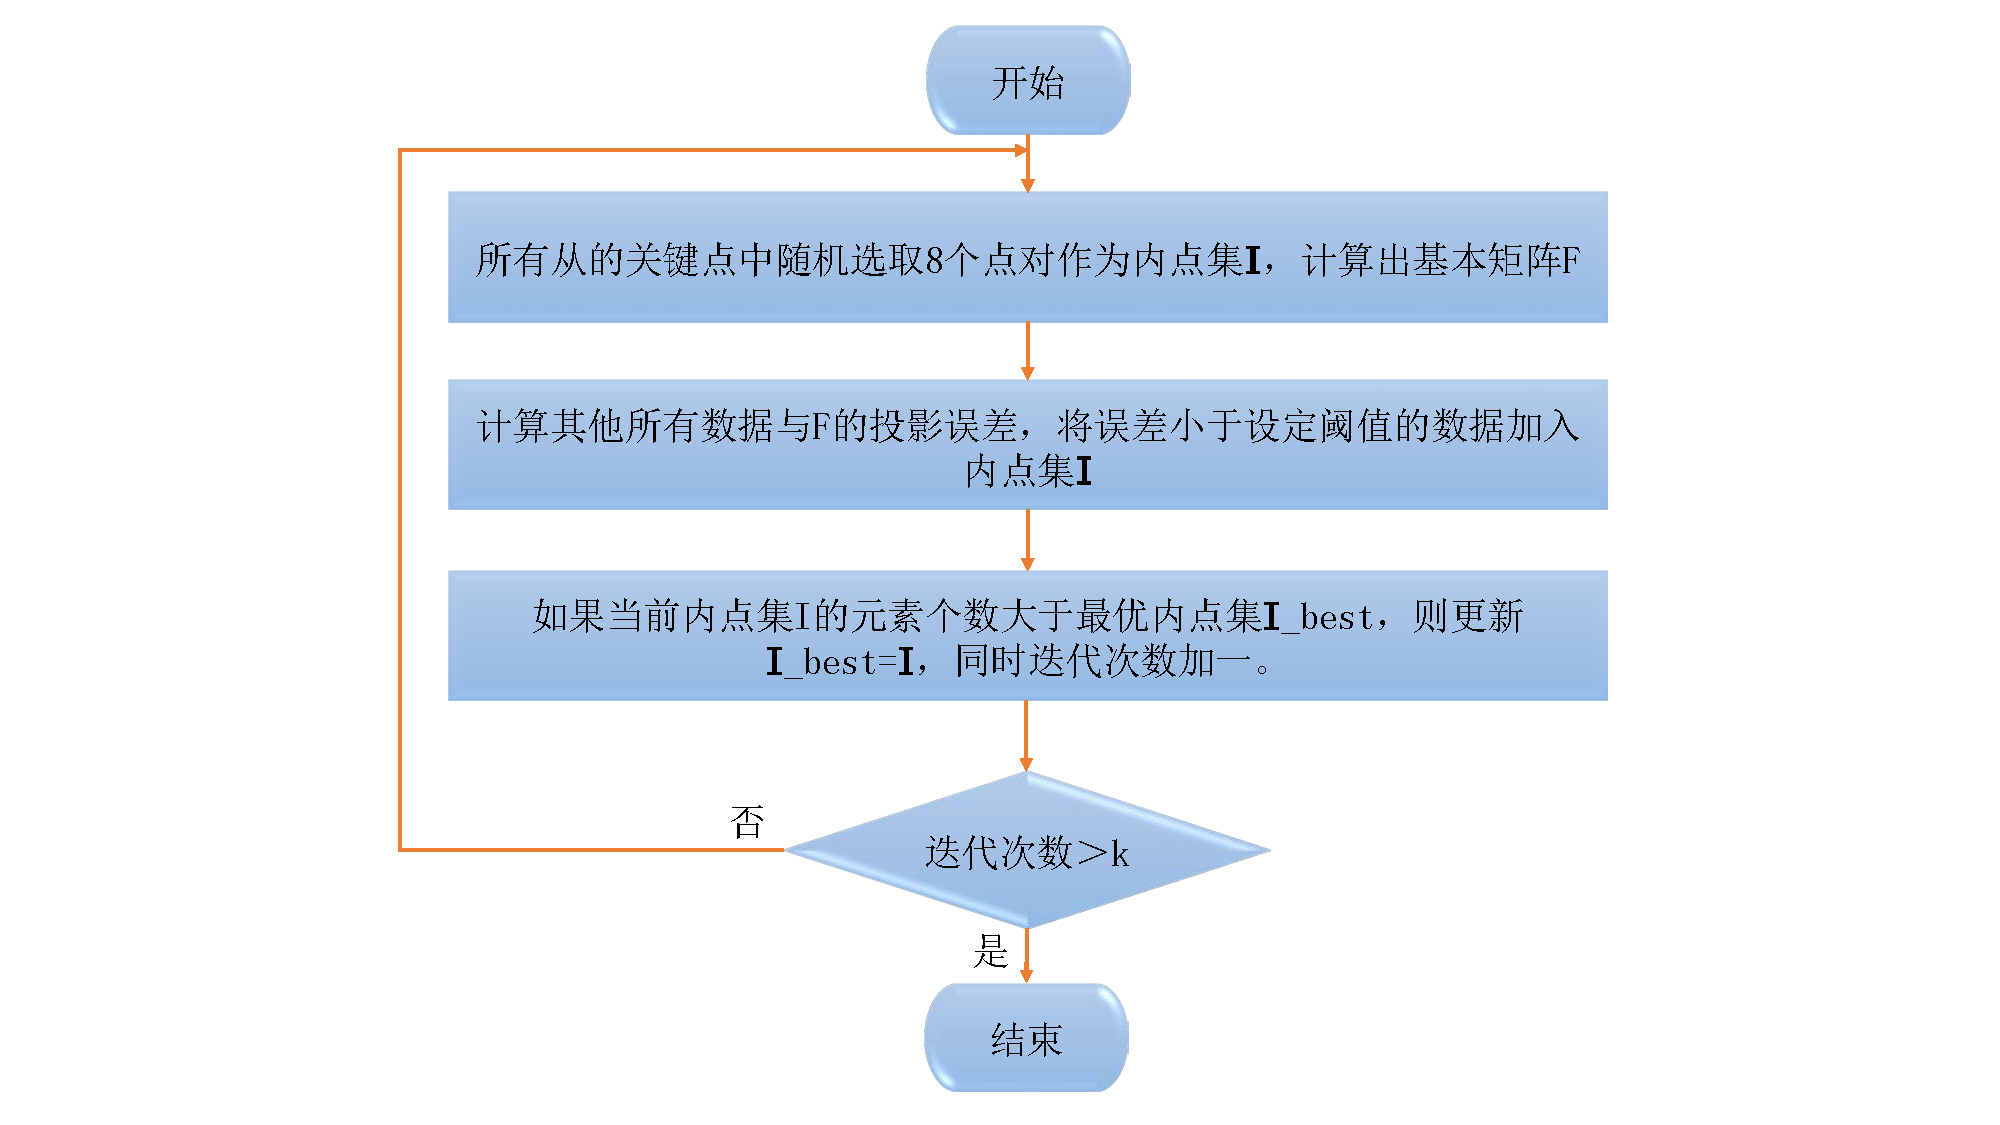
\includegraphics[width=0.65\textwidth]{figures/chapter3/fig3_5}
	\caption{用基本矩阵剔除异常点}\label{fig3_5}
\end{figure}

图\ref{fig3_6}是异常点剔除前后对比图。其中,图(a)是LK光流跟踪到的FAST角点(没有进行异常点剔除),总共1270个点;图(b)是经过异常点剔除后的跟踪的角点,总共775个点。
\begin{figure}[h]\setlength{\belowcaptionskip}{-12pt}
\centering
	\subfigure[剔除前]{
	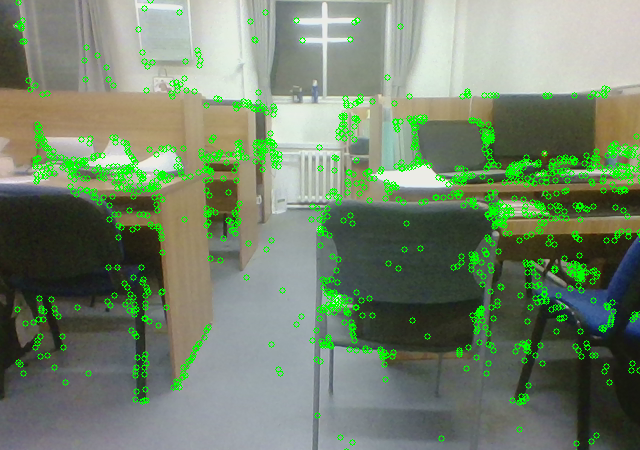
\includegraphics[width=0.4\textwidth]{figures/chapter3/RAN1}}
	\subfigure[剔除后]{
	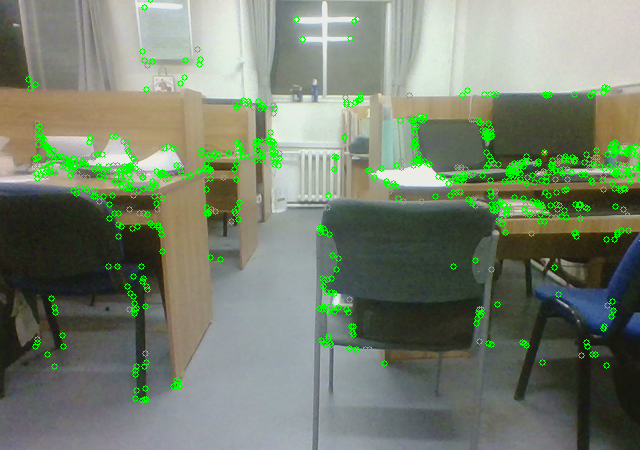
\includegraphics[width=0.4\textwidth]{figures/chapter3/RAN2}}
	\caption{异常点剔除}\label{fig3_6}
\end{figure}
\section{IMU预积分}
通常情况下,IMU的数据频率要远大于相机的数据频率,不可能计算每一个IMU时刻状态量,为了与视觉进行融合,需要提前对相邻视觉帧之间的IMU数据进行积分,这个步骤称为预积分\upcite{forster2015imu}\upcite{shen2015tightly}。图\ref{fig3_7}是预积分示意图。
\begin{figure}[h]\setlength{\belowcaptionskip}{-12pt}
	\centering
	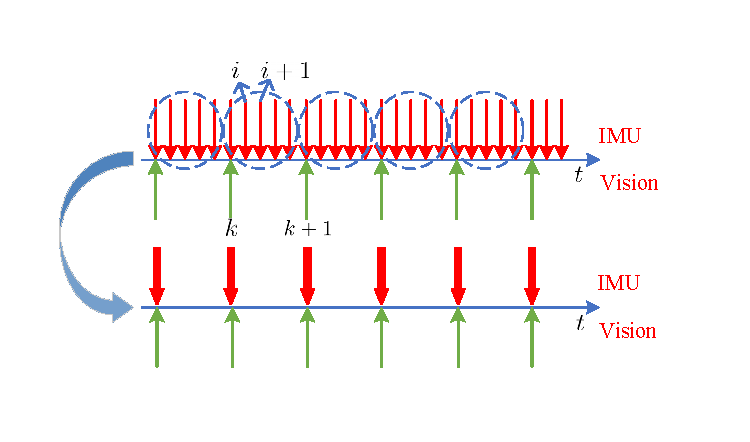
\includegraphics[width=0.3\textwidth, angle=-90]{figures/chapter3/fig3_7}
	\caption{预积分示意图}\label{fig3_7}
\end{figure}

首先定义本节使用得符号和坐标系。定义 $\left(\cdot\right)^w $ 是世界坐标系。重力的方向与世界坐标系的 $z$ 轴对齐。 $\left(\cdot\right)^b $是本体坐标系,本文把它定义为与IMU坐标系相同。 $\left(\cdot\right)^c $ 是相机坐标系。$\mathbf{q}_b^w $ ,$\mathbf{p}_b^w $ 是从本体坐标系到世界坐标系的旋转和平移。$b_k $ 是第 $k$ 个图像对应的本体帧(IMU帧)。 $c_k$ 是第 $k$ 个相机帧。$\otimes  $ 表示两个四元数之间的乘法运算。在世界坐标系下 $\mathbf{g}^w=[0,0,g]^T $ 。 $\hat{\left(\cdot\right)} $ 表示为某一量的噪声测量值或估计值。
\subsection{当前帧的位置、速度和姿态}
假设图像的第 $k+1$  帧为当前帧,根据2.1.3小结研究的IMU状态模型,将图像的第 $k$  帧和第 $k+1$  帧之间的IMU进行积分,得到第 $k+1$ 帧的IMU位置、速度和姿态。
\begin{equation}
\label{eqn:3.13}
\begin{split}
\mathbf{p}_{b_{k+1}}^w&=\mathbf{p}_{b_k}^w+\mathbf{v}_{b_k}^w\Delta t_k+\iint_{t\in[t_k,t_{k+1}]}(\mathbf{R}_t^w(\hat{\mathbf{a}}_t-\mathbf{b}_{a_t}-\mathbf{n}_a)-\mathbf{g}^w)dt^2 \\
\mathbf{v}_{b_{k+1}}^w&=\mathbf{v}_{b_k}^w+\int_{t\in[t_k,t_{k+1}]}(\mathbf{R}_t^w(\hat{\mathbf{a}}_t-\mathbf{b}_{a_t}-\mathbf{n}_a)-\mathbf{g}^w)dt \\
\mathbf{q}_{b_{k+1}}^w&=\mathbf{q}_{b_k}^w \otimes \int_{t\in[t_k,t_{k+1}]}\frac{1}{2}\bm{\Omega}(\hat{\bm{\omega}}_t-\mathbf{b}_{w_t}-\mathbf{n}_w)\mathbf{q}_t^{b_k}dt,
\end{split}
\end{equation}
其中,$\mathbf{R}_t^w $ 表示从IMU坐标系到世界坐标系的变换,与式(\ref{eqn:2.43})中的 $\mathbf{R}_w^t $ 正好相反。

式(\ref{eqn:3.13})是当前帧的位置、速度和姿态的连续表达形式,在实际工程中,为了方便编程,需要离散的形式。使用中值法对式(\ref{eqn:3.13})进行离散化,得,
\begin{equation}
\label{eqn:3.14}
\begin{split}
\mathbf{p}_{{i+1}}^w&=\mathbf{p}_{i}^w+\mathbf{v}_{i}^w\delta t+\frac{1}{2} \overline{\hat{\mathbf{a}}}_{l} \delta t ^{2} \\
\mathbf{v}_{{i+1}}^w&=\mathbf{v}_{i}^w+ \overline{\hat{\mathbf{a}}}_{l} \delta t^{2}\\
\mathbf{q}_{{i+1}}^w&=\mathbf{q}_{i}^w\otimes \begin{bmatrix} 1\\ \frac{1}{2} \overline{\hat{\bm{\omega}}}_{l} \delta t\end{bmatrix},
\end{split}
\end{equation}
其中,
\begin{equation}
\label{eqn:3.15}
\begin{aligned}
\overline{\hat{\mathbf{a}}}_{l} &= \frac{1}{2}\left[\mathbf{q}_{i}\left(\hat{ \mathbf{a}}_{i}-\mathbf{b}_{a_{i}}\right)-\mathbf{g}^{w}+\mathbf{q}_{i+1}\left(\hat{\mathbf{a}}_{i+1}-\mathbf{b}_{a_{i}}\right)-\mathbf{g}^{w}\right] \\ 
\overline{\hat{{\bm{\omega}}}}_{l}   &= \frac{1}{2}\left(\hat{\bm{\omega}}_{i}+\hat{\bm{\omega}}_{i+1}\right)-\mathbf{b}_{\omega_{i}}
\end{aligned}
\end{equation}
$i$ 是与$[t_k,t_{k+1}] $ 内的IMU时刻,$\delta t $ 是时间间隔。
\subsection{两帧之间的位置、速度和姿态增量}
观察式(\ref{eqn:3.13}),发现积分项中包含第 $k$  帧的 $v$ 和 $\mathbf{R}_t^w $ ,也就是第 $k$ 帧的速度和相机相对世界坐标系的旋转,这样将导致三个问题:

(1)这样就相当于将相机位姿耦合到了积分中,如果需要对 $k+1$ 帧的相机的位姿求导,那么需要通过链式法则对 $k+1$ 帧之前的所有位姿进行求导,这样将极大的增加计算量;

(2)在进行非线性优化的时候,每一次优化都会改变状态量,这样就需要重新进行状态传播,同样会增加计算量;

(3) $\mathbf{R}_t^w $实际上是需要求解的未知量。

为了解决上述问题,考虑将优化的状态量从第 $k$ 帧到第 $k+1$ 帧的积分项中提取出来,并将参考坐标系从世界坐标系变化为IMU坐标系。在公式(3.13)的等式两边同时乘以 $\mathbf{R}_w^{b_k} $ ,得,
\begin{equation}
\label{eqn:3.16}
\begin{split}
\mathbf{R}_w^{b_k}\mathbf{p}_{b_{k+1}}^w&=\mathbf{R}_w^{b_k}(\mathbf{p}_{b_k}^w+\mathbf{v}_{b_k}^w\Delta t_k -\frac{1}{2}\mathbf{g}^w\Delta {t_k^2})+\bm{\alpha}_{b_{k+1}}^{b_k} \\
\mathbf{R}_w^{b_k}\mathbf{v}_{b_{k+1}}^w&=\mathbf{R}_w^{b_k}(\mathbf{v}_{b_k}^w-\mathbf{g}^w\Delta t_k)+\bm{\beta}_{b_{k+1}}^{b_k} \\
\mathbf{q}_w^{b_k}\otimes\mathbf{q}_{b_{k+1}}^w&=\bm{\gamma}_{b_{k+1}}^{b_k},
\end{split}
\end{equation}
其中,
\begin{equation}
\label{eqn:3.17}
\begin{split}
\bm{\alpha}_{b_{k+1}}^{b_k}&=\iint_{t\in[t_k,t_{k+1}]}\mathbf{R}_t^{b_k}(\hat{\mathbf{a}}_t-\mathbf{b}_{a_t}-\mathbf{n}_a)dt^2 \\
\bm{\beta}_{b_{k+1}}^{b_k}&=\int_{t\in[t_k,t_{k+1}]}\mathbf{R}_t^{b_k}(\hat{\mathbf{a}}_t-\mathbf{b}_{a_t}-\mathbf{n}_a)dt \\
\bm{\gamma}_{b_{k+1}}^{b_k}&=\iint_{t\in[t_k,t_{k+1}]}\frac{1}{2}\bm{\Omega}(\hat{\bm{\omega}}_t-\mathbf{b}_{w_t}-\mathbf{n}_w)\bm{\gamma}_{t}^{b_k}dt.
\end{split}
\end{equation}
与式(\ref{eqn:3.13})不同的是,式(\ref{eqn:3.17})积分出来的是两帧图像之间IMU的增量信息,而式(\ref{eqn:3.13})给出的是当前帧的位置、速度和姿态信息。称式(\ref{eqn:3.17})为预积分公式,可以看到预积分项只通过IMU测量值就能得到,$b_k $ 变为参考帧。$\bm{\alpha}_{b_{k+1}}^{b_k},\bm{\beta}_{b_{k+1}}^{b_k}, \bm{\gamma}_{b_{k+1}}^{b_k}  $ 只与 $b_{k} $ 和 $b_{k+1} $ 中的IMU偏置bias有关,与其他状态量无关。当bias估计变化很小时,假设 $\bm{\alpha}_{b_{k+1}}^{b_k},\bm{\beta}_{b_{k+1}}^{b_k}, \bm{\gamma}_{b_{k+1}}^{b_k}  $ 与bias是线性关系,可以按其对bias的一阶近似来调整,
\begin{equation}
\label{eqn:3.18}
\begin{aligned}
\bm{\alpha}_{b_{k+1}}^{b_{k}} & \approx \hat{\bm{\alpha}}_{b_{k+1}}^{b_{k}}+\bm{J}_{{b}_{a}}^{\alpha} \delta \mathbf{b}_{a}+\bm{J}_{{b}_{\omega}}^{\alpha} \delta \mathbf{b}_{\omega} \\  
\bm{\beta}_{b_{k+1}}^{b_{k}}  & \approx \hat{\bm{\beta}}_{b_{k+1}}^{b_{k}}+\bm{J}_{b_{a}}^{\beta} \delta \mathbf{b}_{a} + \bm{J}_{b_{\omega}}^{\beta} \delta \mathbf{b}_{\omega} \\
\bm{\gamma}_{b_{k+1}}^{b_{k}} & \approx \hat{\bm{\gamma}}_{b_{k+1}}^{b_{k}} \otimes\left[\frac{1}{2} \bm{J}_{b_{\omega}}^{\gamma} \delta \mathbf{b}_{\omega}\right]
\end{aligned}
\end{equation}
其中得Jacobian矩阵计算及含义参考\ref{chap:3.2.3}小节中的递推公式(\ref{eqn:3.38})和(\ref{eqn:3.40})。否则就进行重新传播。这种方法为基于非线性优化的算法节省了大量的计算资源。

在开始时,$\bm{\alpha}_{b_k}^{b_k},\bm{\beta}_{b_k}^{b_k} $ 是0,$\bm{\gamma}_{b_k}^{b_k} $ 是单位四元数。注意,噪声项 $\mathbf{n}_a,\mathbf{n}_w $ 是未知的,在实现中被视为零,所以这里使用预积分的估计值,记为 $\hat{(\cdot)} $ 。仍然使用中值法对式(\ref{eqn:3.18})进行离散化,得,
\begin{equation}
\label{eqn:3.19}
\begin{aligned}
\hat{\bm{\alpha}}_{i+1}^{b_{k}} &= \hat{\bm{\alpha}}_{i}^{b_{k}}+\hat{\bm{\beta}}_{i}^{b_{k}} \delta t+\frac{1}{2} \overline{\hat{\mathbf{a}}}_{l} \delta t^{2} \\
\hat{\bm{\beta}}_{i+1}^{b_{k}}  &= \hat{\bm{\beta}}_{i}^{b_{k}}+\overline{\hat{\mathbf{a}}}_{l} \delta t \\
\hat{\bm{\gamma}}_{i+1}^{b_{k}} &= \hat{\bm{\gamma}}_{i}^{b_{k}} \otimes \hat{\bm{\gamma}}_{i+1}^{i}=\hat{\bm{\gamma}}_{i}^{b_{k}} \otimes \begin{bmatrix} 1\\ \frac{1}{2} \overline{\hat{\bm{\omega}}}_{l} \delta t\end{bmatrix},
\end{aligned}
\end{equation}
其中,
\begin{equation}
\label{eqn:3.20}
\begin{aligned}
\overline{\hat{\mathbf{a}}}_{l} &= \frac{1}{2}\left[\mathbf{q}_{i}\left(\hat{ \mathbf{a}}_{i}-\mathbf{b}_{a_{i}}\right) +\mathbf{q}_{i+1}\left(\hat{\mathbf{a}}_{i+1}-\mathbf{b}_{a_{i}}\right) \right] \\ 
\overline{\hat{{\bm{\omega}}}}_{l}   &= \frac{1}{2}\left(\hat{\bm{\omega}}_{i}+\hat{\bm{\omega}}_{i+1}\right)-\mathbf{b}_{\omega_{i}}
\end{aligned}
\end{equation}
\subsection{误差状态传播}
\label{chap:3.2.3}
IMU在两个图像帧之间积分出来的值是有误差的,然后研究IMU误差传播过程。IMU的误差状态量为 $[ \delta{\bm{\alpha}}_t^{b_k},\delta{\bm{\beta}}_t^{b_k},
\delta{\bm{\theta}}_t^{b_k} ,\delta{\mathbf{b}}_{a_t} ,\delta{\mathbf{b}}_{w_t} ] ^T$ ,易得:
\begin{equation}
\label{eqn:3.21}
\delta \dot{\bm{\alpha}}_t^{b_k} = \delta \bm{\beta}_t^{b_k}
\end{equation}
由式(\ref{eqn:2.45})得,
\begin{equation}
\label{eqn:3.22}
\begin{aligned}
\delta \dot{\mathbf{b}}_{a_t} &= \mathbf{n}_{b_a} \\
\delta \dot{\mathbf{b}}_{w_t} &= \mathbf{n}_{b_w}
\end{aligned}
\end{equation}
用 $(\cdot)_{true} $ 表示包含噪声的真实测量值,$(\cdot)_{nominal} $ 表示无噪声的理论值。为了方便书写和表达,下面将 $\delta \dot{\bm{\beta}}_t^{b_k}  $ 和 $\delta \dot{\bm{\theta}}_t^{b_k}  $ 分别简写成 $\delta \dot{\bm{\beta}} $ 和 $\delta \dot{\bm{\theta}} $ 则,
\begin{equation}
\label{eqn:3.23}
\delta \dot{\bm{\beta}} = \dot{\bm{\beta}}_{true} - \dot{\bm{\beta}}_{norminal}
\end{equation}
其中,
\begin{equation}
\label{eqn:3.24}
\begin{aligned}
\dot{\bm{\beta}}_{true} &= \hat{\mathbf{R}}_{t_{true}}^{b_k} ( \hat{\mathbf{a}}_{t_{true}} - \mathbf{b}}_{a_{t_{true}}) \\
&= \mathbf{R}_t^{b_k} \text{Exp}( [\delta \bm{\theta}]_{\times} ) ( \hat{\mathbf{a}}_t - \mathbf{n}_a - \mathbf{b}_{a_t} - \delta\mathbf{b}_{a_t} ) \\
&= \mathbf{R}_t^{b_k} (\mathbf{I}+[\delta \bm{\theta}]_{\times} )(\hat{\mathbf{a}}_t - \mathbf{n}_a - \mathbf{b}_{a_t} - \delta\mathbf{b}_{a_t}  ) \\
&= \mathbf{R}_t^{b_k} ( \hat{\mathbf{a}}_t - \mathbf{n}_a - \mathbf{b}_{a_t} - \delta\mathbf{b}_{a_t} + [\delta \bm{\theta}]_{\times} (\hat{\mathbf{a}}_t - \mathbf{b}_{a_t} )) \\
&= \mathbf{R}_t^{b_k} ( \hat{\mathbf{a}}_t - \mathbf{n}_a - \mathbf{b}_{a_t} - \delta\mathbf{b}_{a_t} - [(\hat{\mathbf{a}}_t - \mathbf{b}_{a_t}) ]_{\times} \delta \bm{\theta} ) 
\end{aligned}
\end{equation}
\begin{equation}
\label{eqn:3.25}
\dot{\bm{\beta}}_{norminal} = \mathbf{R}_t^{b_k}(\hat{\mathbf{a}}_t-\mathbf{b}_{a_t})
\end{equation}
将式(\ref{eqn:3.23})、(\ref{eqn:3.24})代入式(\ref{eqn:3.25})得,
\begin{equation}
\label{eqn:3.26}
\begin{aligned}
\delta \dot{\bm{\beta}} &= \dot{\bm{\beta}}_{true}-\dot{\bm{\beta}}_{nominal} \\
&= -\mathbf{R}_{t}^{b_{k}} [\left(\hat{\mathbf{a}}_{t}-\mathbf{b}_{a_{t}}\right)]_{\times} \delta \theta - \mathbf{R}_{t}^{b_{k}} \delta \mathbf{b}_{a_{t}} - \mathbf{R}_{t}^{b_{k}} \mathbf{n}_{a}
\end{aligned}
\end{equation}
由式(\ref{eqn:2.42})可得,
\begin{equation}
\label{eqn:3.27}
\begin{aligned}
\dot{\mathbf{q}}_{true} &= \frac{1}{2} \mathbf{q}_{t_{true}} \otimes \left[ \begin{array}{c}{\bm{\omega}_{true}} \\ {0}\end{array}\right] \\
&= \frac{1}{2} \mathbf{q}_{t} \otimes \delta \mathbf{q} \otimes \left[ \begin{array}{c}{\hat{\bm{\omega}}_{t}-\mathbf{b}_{\omega_{t}}-\mathbf{n}_{\omega}-\delta \mathbf{b}_{\omega_{t}}} \\ {0}\end{array}\right]
\end{aligned}
\end{equation}
由四元数导数性质可得,
\begin{equation}
\label{eqn:3.28}
\begin{aligned}
\dot{\mathbf{q}}_{true} &= \dot{(\mathbf{q}_{t} \otimes \delta \mathbf{q}) } \\
&= \dot{\mathbf{q}}_{t} \otimes \delta \mathbf{q} + \mathbf{q}_{t} \otimes \dot{\delta \mathbf{q}} \\
&= \frac{1}{2} \mathbf{q}_{t} \otimes \left[ \begin{array}{c}{\hat{\bm{\omega}}_{t}-\mathbf{b}_{\omega_{t}}} \\ {0}\end{array}\right] \otimes \delta \mathbf{q}+\mathbf{q}_{t} \otimes \dot{\delta \mathbf{q}} 
\end{aligned}
\end{equation}
联立式(\ref{eqn:3.27})、(\ref{eqn:3.28})可得,
\begin{equation}
\label{eqn:3.29}
\begin{aligned}
&  \frac{1}{2} \mathbf{q}_{t} \otimes \delta \mathbf{q} \otimes \left[ \begin{array}{c}{\hat{\bm{\omega}}_{t}-\mathbf{b}_{\omega_{t}}-\mathbf{n}_{\omega}-\delta \mathbf{b}_{\omega_{t}}} \\ {0}\end{array}\right]
= \frac{1}{2} \mathbf{q}_{t} \otimes \left[ \begin{array}{c}{\hat{\bm{\omega}}_{t}-\mathbf{b}_{\omega_{t}}} \\ {0}\end{array}\right] \otimes \delta \mathbf{q}+\mathbf{q}_{t} \otimes \dot{\delta \mathbf{q}} \\   
& \Leftrightarrow \quad \frac{1}{2} \delta \mathbf{q} \otimes \left[ \begin{array}{c}{\hat{\bm{\omega}}_{t}-\mathbf{b}_{\omega_{t}}-\mathbf{n}_{\omega}-\delta \mathbf{b}_{\omega_{t}}} \\ {0}\end{array}\right]
= \frac{1}{2} \left[ \begin{array}{c}{\hat{\bm{\omega}}_{t}-\mathbf{b}_{\omega_{t}}} \\ {0}\end{array}\right] \otimes \delta \mathbf{q}+\mathbf{q}_{t} \otimes \dot{\delta \mathbf{q}} \\
& \Leftrightarrow \quad 2\dot{\delta \mathbf{q}} = \delta \mathbf{q} \otimes \left[ \begin{array}{c}{\hat{\bm{\omega}}_{t}-\mathbf{b}_{\omega_{t}}-\mathbf{n}_{\omega}-\delta \mathbf{b}_{\omega_{t}}} \\ {0}\end{array}\right]
- \left[ \begin{array}{c}{\hat{\bm{\omega}}_{t}-\mathbf{b}_{\omega_{t}}} \\ {0}\end{array}\right] \otimes \delta \mathbf{q} \\
& \Leftrightarrow \quad 2\dot{\delta \mathbf{q}} = \left[\left[ \begin{array}{c}{\hat{\bm{\omega}}_{t}-\mathbf{b}_{\omega_{t}}-\mathbf{n}_{\omega}-\delta \mathbf{b}_{\omega_{t}}} \\ {0}\end{array}\right]\right]_R \delta \mathbf{q}
- \left[\left[ \begin{array}{c}{\hat{\bm{\omega}}_{t}-\mathbf{b}_{\omega_{t}}} \\ {0}\end{array}\right]\right]_L \delta \mathbf{q} \\
& \Leftrightarrow \quad 2\dot{\delta \mathbf{q}} = 
\left[ \begin{array}
{cc}{-\left[2 \hat{\bm{\omega}}_{t}-2 \mathbf{b}_{\omega_{t}}-\mathbf{n}_{\omega}-\delta \mathbf{b}_{\omega_{t}}\right]_\times} & {-\mathbf{n}_{\omega}-\delta \mathbf{b}_{\omega_{t}}} \\ 
{\left(\mathbf{n}_{\omega}+\delta \mathbf{b}_{\omega_{t}}\right)^{T}} & {\bm{0}}
\end{array}\right]
\begin{bmatrix}
\frac{\delta \bm{\theta}}{2} \\
1
\end{bmatrix},
\end{aligned}     
\end{equation}
又因为,
\begin{equation}
\label{eqn:3.30}
2 \dot{\delta} \mathbf{q}= \left[ \begin{array}{c}{\dot{\delta} \bm{\theta}} \\ {0}\end{array}\right]
\end{equation}
所以,
\begin{equation}
\label{eqn:3.31}
\left[ \begin{array}{c}{\dot{\delta} \bm{\theta}} \\ {0}\end{array}\right]
=\left[ \begin{array}
{cc}{ -\left[2 \hat{\bm{\omega}}_{t}-2 \mathbf{b}_{\omega_{t}}-\mathbf{n}_{\omega}-\delta \mathbf{b}_{\omega_{t}}\right]_\times } & {-\mathbf{n}_{\omega}-\delta \mathbf{b}_{\omega_{t}}} \\ 
{\left(\mathbf{n}_{\omega}+\delta \mathbf{b}_{\omega_{t}}\right)^{T}} & {\bm{0}}
\end{array}\right]
\begin{bmatrix}
\frac{\delta \bm{\theta}}{2} \\
1
\end{bmatrix},   
\end{equation}
从而得到 $\dot{\delta \bm{\theta} }$ 得表达式,
\begin{equation}
\label{eqn:3.32}
\begin{aligned}
\dot{\delta \bm{\theta}} &=
-\left[2 \hat{\bm{\omega}}_{t}-2 \mathbf{b}_{\omega_{t}}-\mathbf{n}_{\omega}-\delta \mathbf{b}_{\omega_{t}}\right]_\times \frac{\delta \bm{\theta}}{2}-\mathbf{n}_{\omega}-\delta \mathbf{b}_{\omega_{t}} \\
& \approx-\left[\hat{\bm{\omega}}_{t}-\mathbf{b}_{\omega_{t}}\right]_\times \delta \bm{\theta}-\mathbf{n}_{\omega}-\delta \mathbf{b}_{\omega_{t}}
\end{aligned}
\end{equation}
由式(\ref{eqn:3.21})、(\ref{eqn:3.22})、(\ref{eqn:3.26})和(\ref{eqn:3.32})可得IMU预积分在 $t$ 时刻误差项得导数为:
\begin{equation}
\label{eqn:3.33}
\begin{split}
\begin{bmatrix}
\delta\dot{\bm{\alpha}}_t^{b_k} \\
\delta\dot{\bm{\beta }}_t^{b_k} \\
\delta\dot{\bm{\theta}}_t^{b_k} \\
\delta\dot{\mathbf{b}}_{a_t} \\
\delta\dot{\mathbf{b}}_{w_t} \\
\end{bmatrix} &= 
\begin{bmatrix}
0 & \mathbf{I} & 0 & 0 & 0 \\
0 & 0 & -\mathbf{R}_t^{b_k}\left[{\hat{\mathbf{a}}_t-\mathbf{b}_{a_t}}\right]_\times & -\mathbf{R}_t^{b_k} & 0 \\
0 & 0 & -\left[{\hat{\bm{\omega}}_t-\mathbf{b}_{w_t}}\right]_\times & 0 & -\mathbf{I} \\
0 & 0 & 0 & 0 & 0 \\
0 & 0 & 0 & 0 & 0 \\
\end{bmatrix}
\begin{bmatrix}
\delta\bm{\alpha}_t^{b_k} \\
\delta\bm{\beta }_t^{b_k} \\
\delta\bm{\theta}_t^{b_k} \\
\delta\mathbf{b}_{a_t} \\
\delta\mathbf{b}_{w_t} \\
\end{bmatrix} \\
&+\begin{bmatrix}
0 & 0 & 0 & 0 \\
-\mathbf{R}_t^{b_k} & 0 & 0 & 0 \\
0 & -\mathbf{I} & 0 & 0  \\
0 & 0 & \mathbf{I} & 0 \\
0 & 0 & 0 & \mathbf{I} \\
\end{bmatrix}
\begin{bmatrix}
\mathbf{n}_a \\ \mathbf{n}_w \\ 
\mathbf{n}_{b_a} \\ \mathbf{n}_{b_w}
\end{bmatrix} = \mathbf{F}_t \delta \mathbf{z}_t^{b_k}
+\mathbf{G}_t\mathbf{n}_t,
\end{split}
\end{equation}

式(\ref{eqn:3.33})是式(\ref{eqn:3.17})在连续时间下的IMU误差状态方程,其中,$ \mathbf{F}_t $ 是15×15维,$ \mathbf{G}_t $ 是15×12维,$ \delta \mathbf{z}_t^{b_k}$ 是15×1维,$\mathbf{n}_t $ 是12×1维。

将式(\ref{eqn:3.33})简写为:
\begin{equation}
\label{eqn:3.34}
\dot{\delta \mathbf{z}}_t^{b_k} = \mathbf{F}_t \delta \mathbf{z}_t^{b_k} + \mathbf{G}_t\mathbf{n}_t
\end{equation}
由导数定义知,
\begin{equation}
\label{eqn:3.35}
\dot{\delta \mathbf{z}}_t^{b_k} = \lim _{\delta t \rightarrow 0} \frac{\delta \mathbf{z}_{t+\delta t}^{b_k} - \delta \mathbf{z}_t^{b_k}}{\delta t}
\end{equation}
所以,
\begin{equation}
\label{eqn:3.36}
\delta \mathbf{z}_{t+\delta t}^{b_k} = \delta \mathbf{z}_t^{b_k} + \dot{\delta \mathbf{z}}_t^{b_k} \delta t
\end{equation}
将式(\ref{eqn:3.34})代入式(\ref{eqn:3.36})得,
\begin{equation}
\label{eqn:3.37}
\setlength{\abovedisplayskip}{6pt}
\setlength{\belowdisplayskip}{6pt}
\delta \mathbf{z}_{t+\delta t}^{b_k} = ( \mathbf{I}+ \mathbf{F}_t \delta t )\delta \mathbf{z}_t^{b_k} + ( \mathbf{G}_t \delta t )\mathbf{n}_t
\end{equation}
式(\ref{eqn:3.37})表示当前时刻IMU的预积分误差与上一时刻的IMU的预积分误差成线性关系,将式(\ref{eqn:3.37})与扩展卡尔曼滤波的运动方程对比发现,其与EKF对非线性系统线性化的过程如出一辙。所以,可以根据当前时刻IMU预积分的误差预测出下一时刻IMU预积分的误差的均值和协方差。均值预测可以通过式(\ref{eqn:3.37})计算,而协方差预测公式可以类比EKF协方差更新公式得到,
\begin{equation}
\label{eqn:3.38}
\setlength{\abovedisplayskip}{6pt}
\setlength{\belowdisplayskip}{6pt}
\mathbf{P}_{t+\delta t}^{b_k}=(\mathbf{I}+\mathbf{F}_t\delta t)\mathbf{P}_t^{b_k}(\mathbf{I}+\mathbf{F}_t\delta t)^T+(\mathbf{G}_t\delta t)\mathbf{Q}(\mathbf{G}_t\delta t)^T
\end{equation}
协方差初始值 $\mathbf{P}_{b_k}^{b_k}=0 $ ,其中 $\mathbf{Q} $ 是噪声的对角线协方差矩阵,维数为12×12,
\begin{equation}
\label{eqn:3.39}
\mathbf{Q} =\left[ \begin{array}{cccc}
{\bm{\sigma}_{a}^{2}} & {0} & {0} & {0} \\ 
{0} & {\bm{\sigma}_{w}^{2}} & {0} & {0} \\ 
{0} & {0} & {\bm{\sigma}_{b_{a}}^{2}} & {0} \\ 
{0} & {0} & {0} & {\bm{\sigma}_{b_{w}}^{2}
}\end{array}\right]
\end{equation}

由公式(\ref{eqn:3.37})可以得到误差项的Jacobian递归计算公式, 
\begin{equation}
\label{eqn:3.40}
\setlength{\abovedisplayskip}{6pt}
\setlength{\belowdisplayskip}{6pt}
\mathbf{J}_{t+\delta t}=(\mathbf{I}+\mathbf{F}_t\delta t)\mathbf{J}_t
\end{equation}
其中,$\mathbf{J} $ 的初始值为 $\mathbf{J}_{b_k}=\mathbf{I}  $ 。

利用递推公式(\ref{eqn:3.38})和(\ref{eqn:3.40}),可以得到协方差矩阵 $\mathbf{p}_{b_{k+1}}^{b_k}  $ 和雅可比矩阵 $\mathbf{J}_{b_{k+1}} $ 。 $\bm{\alpha}_{b_{k+1}}^{b_k},\bm{\beta}_{b_{k+1}}^{b_k}, \bm{\gamma}_{b_{k+1}}^{b_k} $ 关于偏置的一阶近似可以写成公式(\ref{eqn:3.18})的形式。公式(\ref{eqn:3.18})中 $ \mathbf{J}_{b_a}^\alpha $ 是 $ \mathbf{J}_{b_{k+1}} $ 中的分块矩阵,其位置对应于 $ {\delta\alpha_{b_{k+1}}^{b_k}}/{\delta b_{a_k}} $ , $ \mathbf{J}_{b_w}^\alpha,\mathbf{J}_{b_a}^\beta,\mathbf{J}_{b_w}^\beta,\mathbf{J}_{b_w}^\gamma. $ 类似,不再累述。当bias估计发生轻微变化时,使用公式(\ref{eqn:3.18})近似校正预积分结果,而不是重新传播。

下面写出IMU的预积分测量模型:
\begin{equation}
\label{eqn:3.41}
\begin{bmatrix}
\hat{\bm{\alpha}}_{b_{k+1}}^{b_k} \\ \hat{\bm{\beta}}_{b_{k+1}}^{b_k} \\ \hat{\bm{\gamma}}_{b_{k+1}}^{b_k} \\ 0 \\ 0
\end{bmatrix}=
\begin{bmatrix}
\mathbf{R}_w^{b_k}(\mathbf{p}_{b_{k+1}}^w-\mathbf{p}_{b_k}^w+\frac{1}{2}\mathbf{g}^w\Delta t_k^2-\mathbf{v}_{b_k}^w\Delta t_k) \\ \mathbf{R}_w^{b_k}(\mathbf{v}_{b_{k+1}}^w+\mathbf{g}^w\Delta t_k-\mathbf{v}_{b_k}^w) \\ \mathbf{q}_{b_k}^{w^{-1}}\otimes \mathbf{q}_{b_{k+1}}^w \\ \mathbf{b}_{ab_{k+1}}-\mathbf{b}_{ab_k} \\ \mathbf{b}_{wb_{k+1}}-\mathbf{b}_{wb_k}
\end{bmatrix}.
\end{equation}

考虑到实际编程需求,接下来对连续时间下的IMU误差状态方程(\ref{eqn:3.33})进行离散化。设IMU离散化的误差状态量为 $[\delta \bm{\alpha}_{k}, {\delta \bm{\theta}_{k}}, {\delta \bm{\beta}_{k}}, \delta \mathbf{b}_{a_{k}}, \delta \mathbf{b}_{w_{k}}]^T $ 。

式(\ref{eqn:3.32})是角度增量误差导数的连续形式,对其进行离散化,得,
\begin{equation}
\label{eqn:3.42}
\delta \dot{\bm{\theta}}_{k}=-\left[\frac{\hat{\bm{\omega}}_{k}+\hat{\bm{\omega}}_{k+1}}{2}-\mathbf{b}_{\omega_{k}}\right]_\times \delta \bm{\theta}_{k}
-\frac{\mathbf{n}_{\omega_{k}}+\mathbf{n}_{\omega_{k+1}}}{2}-\delta \mathbf{b}_{\omega_{k}}
\end{equation}

根据导数的定义,得到下一时刻的角度增量误差为,
\begin{equation}
\label{eqn:3.43}
\delta \bm{\theta}_{k+1}=\left(\mathbf{I}-\left[\frac{\hat{\bm{\omega}}_{k}+\hat{\bm{\omega}}_{k+1}}{2}-\mathbf{b}_{\omega_{k}}\right]_\times \delta t\right) \delta \bm{\theta}_{k}
- \frac{\mathbf{n}_{\omega_{k}} + \mathbf{n}_{\omega_{k+1}}}{2} \delta t
- \delta t \delta \mathbf{b}_{\omega_{k}}
\end{equation}

式(\ref{eqn:3.26})是速度增量误差导数的连续形式,对其进行离散化,得,
\begin{equation}
\label{eqn:3.44}
\begin{aligned}
\delta \dot{\bm{\beta}}_{k}= & -\frac{1}{2} \mathbf{R}_{k} \left[\hat{\mathbf{a}}_{k}- \mathbf{b}_{a_{k}}\right]_\times \delta \bm{\theta}_{k} 
- \frac{1}{2} \mathbf{R}_{k+1}\left[\hat{\mathbf{a}}_{k+1} - \mathbf{b}_{a_{k}}\right]_\times \delta \bm{\theta}_{k+1} \\
&- \frac{1}{2}\left(\mathbf{R}_{k} + \mathbf{R}_{k+1}\right) \delta \mathbf{b}_{a_{k}}
- \frac{1}{2} \mathbf{R}_{k} \mathbf{n}_{a_{k}}
-\frac{1}{2} \mathbf{R}_{k+1} \mathbf{n}_{a_{k+1}}
\end{aligned}
\end{equation}

将式(\ref{eqn:3.43})代入式(\ref{eqn:3.44})得,
\begin{equation}
\label{eqn:3.45}
\begin{aligned}
\delta \dot{\bm{\beta}}_{k} 
&= -\frac{1}{2} \mathbf{R}_{k}\left[\hat{\mathbf{a}}_{k} - \mathbf{b}_{a_{k}}\right]_\times \delta \bm{\theta}_{k}-\frac{1}{2} \mathbf{R}_{k+1}\left[\hat{\mathbf{a}}_{k+1}-\mathbf{b}_{a_{k}}\right]_\times \\
& \left\{\left[\mathbf{I}- \left[\frac{\hat{\bm{\omega}}_{k}+\hat{\bm{\omega}}_{k+1}}{2}-\mathbf{b}_{\omega_{k}}\right]_\times \delta t\right] \delta \bm{\theta}_{k} 
- \frac{\mathbf{n}_{\omega_{k}}+\mathbf{n}_{\omega_{k+1}}}{2} \delta t-\delta t \delta \mathbf{b}_{\omega_{k}}\right\} \\
& -\frac{1}{2}\left(\mathbf{R}_{k}+\mathbf{R}_{k+1}\right) \delta \mathbf{b}_{a_{k}}-\frac{1}{2} \mathbf{R}_{k} \mathbf{n}_{a_{k}}-\frac{1}{2} \mathbf{R}_{k+1} \mathbf{n}_{a_{k+1}} \\
&= \left\{-\frac{1}{2} \mathbf{R}_{k}\left[\hat{\mathbf{a}}_{k}-\mathbf{b}_{a_{k}}\right]_\times-\frac{1}{2} \mathbf{R}_{k+1}\left[\hat{\mathbf{a}}_{k+1}-\mathbf{b}_{a_{k}}\right]_\times\right. \\
& \left.\left[\mathbf{I}-\left[\frac{\hat{\bm{\omega}}_{k}+\hat{\bm{\omega}}_{k+1}}{2}-\mathbf{b}_{\omega_{k}}\right]_\times \delta t\right]\right\} \delta \bm{\theta}_{k} \\
& +\frac{\delta t}{4} \mathbf{R}_{k+1}\left[\hat{\mathbf{a}}_{k+1}-\mathbf{b}_{a_{k}}\right]_\times \mathbf{n}_{\omega_{k}}+\frac{\delta t}{4} \mathbf{R}_{k+1}\left[\hat{\mathbf{a}}_{k+1}-\mathbf{b}_{a_{k}}\right]_\times \mathbf{n}_{\omega_{k+1}} \\
&+ \frac{\delta t}{2} \mathbf{R}_{k+1}\left[\hat{\mathbf{a}}_{k+1}-\mathbf{b}_{a_{k}}\right]_\times \delta \mathbf{b}_{\omega_{k}} -\frac{1}{2}\left(\mathbf{R}_{k}+\mathbf{R}_{k+1}\right) \delta \mathbf{b}_{a_{k}} \\ 
&-\frac{1}{2} \mathbf{R}_{k} \mathbf{n}_{a_{k}}-\frac{1}{2} \mathbf{R}_{k+1} \mathbf{n}_{a_{k+1}}
\end{aligned}
\end{equation}

根据导数的定义,得到下一时刻的速度增量误差为,
\begin{equation}
\label{eqn:3.46}
\begin{aligned}
\delta \bm{\beta}_{k+1}=& f_{21} \delta \bm{\theta}_{k}+\delta \bm{\beta}_{k}-\frac{1}{2}\left( \mathbf{R}_{k}+\mathbf{R}_{k+1}\right) \delta t \delta \mathbf{b}_{a_{k}}+f_{24} \delta \mathbf{b}_{\omega_{k}} \\ 
& -\frac{1}{2} \mathbf{R}_{k} \delta t \mathbf{n}_{a_{k}} +v_{21} \mathbf{n}_{\omega_{k}}-\frac{1}{2} \mathbf{R}_{k+1} \delta t \mathbf{n}_{a_{k+1}}+v_{23} \mathbf{n}_{\omega_{k+1}}
\end{aligned}
\end{equation}
其中,
\begin{equation}
\label{eqn:3.47}
\begin{aligned}
f_{21} &= -\frac{1}{2} \mathbf{R}_{k}\left[\hat{\mathbf{a}}_{k}-\mathbf{b}_{a_{k}}\right]_\times \delta t \\
& -\frac{1}{2} \mathbf{R}_{k+1}\left[\hat{\mathbf{a}}_{k+1}-\mathbf{b}_{a_{k}}\right]_\times\left[\mathbf{I}-\left[\frac{\hat{\bm{\omega}}_{k}+\hat{\bm{\omega}}_{k+1}}{2}-\mathbf{b}_{\omega_{k}}\right]_\times \delta t\right] \delta t \\
f_{24} &= \frac{1}{2} \mathbf{R}_{k+1}\left[\hat{\mathbf{a}}_{k+1}-\mathbf{b}_{a_{k}}\right]_\times \delta t^{2} \\
v_{21} &= v_{23}=\frac{1}{4} \mathbf{R}_{k+1}\left[\hat{\mathbf{a}}_{k+1}-\mathbf{b}_{a_{k}}\right]_\times \delta t^{2}
\end{aligned}
\end{equation}
由式(\ref{eqn:3.21})知,位置增量误差导数的连续时间形式为,
\begin{equation}
\label{eqn:3.48}
\setlength{\abovedisplayskip}{6pt}
\setlength{\belowdisplayskip}{6pt}
\delta \dot{\bm{\alpha}_k}=\delta \bm{\beta}_k
\end{equation}
对其离散化得,
\begin{equation}
\label{eqn:3.49}
\begin{aligned}
\delta \dot{\bm{\alpha}}_{k} &= \frac{1}{2} \delta \bm{\beta}_{k}+\frac{1}{2} \delta \bm{\beta}_{k+1} \\
&=\delta \bm{\beta}_{k}+\frac{1}{2} f_{21} \delta \bm{\theta}_{k}-\frac{1}{4}\left( \mathbf{R}_{k}+\mathbf{R}_{k+1}\right) \delta t \delta \mathbf{b}_{a_{k}}+\frac{1}{2} f_{24} \delta \mathbf{b}_{\omega_{k}} \\ 
& -\frac{1}{4} \mathbf{R}_{k} \delta t \mathbf{n}_{a_{k}} +\frac{1}{2} v_{21} \mathbf{n}_{\omega_{k}}-\frac{1}{4} \mathbf{R}_{k+1} \delta t \mathbf{n}_{a_{k+1}}+\frac{1}{2} v_{23} \mathbf{n}_{\omega_{k+1}}
\end{aligned}
\end{equation}
根据导数的定义,得到下一时刻的位置增量误差为,
\begin{equation}
\label{eqn:3.50}
\begin{aligned}
\delta \bm{\alpha}_{k+1} =& \delta \bm{\alpha}_{k}+\frac{\delta t}{2} f_{21} \delta \bm{\theta}_{k}+\delta t \delta \bm{\beta}_{k}-\frac{1}{4}\left( \mathbf{R}_{k}+\mathbf{R}_{k+1}\right) \delta t^{2} \delta \mathbf{b}_{a_{k}}+\frac{\delta t}{2} f_{24} \delta \mathbf{b}_{\omega_{k}} \\
& -\frac{1}{4} \mathbf{R}_{k} \delta t^{2} \mathbf{n}_{a_{k}} +\frac{\delta t}{2} v_{21} \mathbf{n}_{\omega_{k}}-\frac{1}{4} \mathbf{R}_{k+1} \delta t^{2} \mathbf{n}_{a_{k+1}}+\frac{\delta t}{2} v_{23} \mathbf{n}_{\omega_{k+1}}
\end{aligned}
\end{equation}
由式(\ref{eqn:2.43})、(\ref{eqn:3.46})和(\ref{eqn:3.50})可得离散形式的IMU增量误差状态方程,
\begin{equation}
\label{eqn:3.51}
\begin{aligned}
\left[ \begin{array}{c}
{\delta \bm{\alpha}_{k+1}} \\ {\delta \bm{\theta}_{k+1}} \\ {\delta \bm{\beta}_{k+1}} \\ {\delta \mathbf{b}_{a_{k+1}}} \\ {\delta \mathbf{b}_{w_{k+1}}}
\end{array}\right]
&=\left[ \begin{array}{ccccc}
\mathbf{I} & {f_{01}} & {\delta t} & {f_{03}} & {f_{04}} \\ 
{0} & {f_{11}} & {0} & {0} & {-\delta t} \\ 
{0} & {f_{21}} & {I} & {f_{23}} & {f_{24}} \\ 
{0} & {0} & {0} & {I} & {0} \\ 
{0} & {0} & {0} & {0} & {I}
\end{array}\right] 
\left[ \begin{array}{c}
{\delta \bm{\alpha}_{k}} \\ {\delta \bm{\theta}_{k}} \\ {\delta \bm{\beta}_k} \\ {\delta \mathbf{b}_{a_{k}}} \\ {\delta \mathbf{b}_{w_{k}}}
\end{array}\right] \\
&+ \left[ \begin{array}{cccccc}
{v_{00}} & {v_{01}} & {v_{02}} & {v_{03}} & {0} & {0} \\ 
{0} & {\frac{-\delta t}{2}} & {0} & {\frac{-\delta t}{2}} & {0} & {0} \\ 
{-\frac{\mathbf{R}_{k} \delta t}{2}} & {v_{21}} & {-\frac{\mathbf{R}_{k+1} \delta t}{2}} & {v_{23}} & {0} & {0} \\ 
{0} & {0} & {0} & {0} & {\delta t} & {0} \\ 
{0} & {0} & {0} & {0} & {0} & {\delta t}\end{array}\right] 
\left[ \begin{array}
{c}{\mathbf{n}_{a_{k}}} \\ {\mathbf{n}_{w_{k}}} \\ {\mathbf{n}_{a_{k+1}}} \\ {\mathbf{n}_{w_{k+1}}} \\ {\mathbf{n}_{b_{a}}} \\ {\mathbf{n}_{b_{w}}}
\end{array}\right]
\end{aligned}
\end{equation}
其中,
\begin{equation}
\label{eqn:3.52}
\left\{
\begin{aligned}
f_{01} &= \frac{\delta t}{2} f_{21} \\
&= -\frac{1}{4} \mathbf{R}_{k}\left[\hat{\mathbf{a}}_{k}-\mathbf{b}_{a_{k}}\right]_\times \delta t^{2}-\frac{1}{4} \mathbf{R}_{k+1}\left[\hat{\mathbf{a}}_{k+1}-\mathbf{b}_{a_{k}}\right]_\times \\ 
& \left[\mathbf{I}-\left[\frac{\hat{\bm{\omega}}_{k}+\hat{\bm{\omega}}_{k+1}}{2}-\mathbf{b}_{\omega_{k}}\right]_\times \delta t\right] \delta t^{2} \\
f_{03} &= -\frac{1}{4}\left(\mathbf{R}_{k}+\mathbf{R}_{k+1}\right) \delta t^{2} \\
f_{04} &= \frac{\delta t}{2} f_{24}=\frac{1}{4} \mathbf{R}_{k+1}\left[\hat{\mathbf{a}}_{k+1}-\mathbf{b}_{a_{k}}\right]_\times \delta t^{3} \\
f_{11} &= I-\left[\frac{\hat{\bm{\omega}}_{k}+\hat{\bm{\omega}}_{k+1}}{2}-\mathbf{b}_{\omega_{k}}\right]_\times \delta t \\
f_{21} &= -\frac{1}{2} \mathbf{R}_{k}\left[\hat{\mathbf{a}}_{k}-\mathbf{b}_{a_{k}}\right]_\times \delta t-\frac{1}{2} \mathbf{R}_{k+1}\left[\hat{\mathbf{a}}_{k+1}-\mathbf{b}_{a_{k}}\right]_\times \\ 
& \left[\mathbf{I}-\left[\frac{\hat{\bm{\omega}}_{k}+\hat{\bm{\omega}}_{k+1}}{2}-\mathbf{b}_{\omega_{k}}\right]_\times \delta t\right] \delta t \\
f_{23} &= -\frac{1}{2}\left(\mathbf{R}_{k}+\mathbf{R}_{k+1}\right) \delta t \\
f_{24} &= \frac{1}{2} \mathbf{R}_{k+1}\left[\hat{\mathbf{a}}_{k+1}-\mathbf{b}_{a_{k}}\right]_\times \delta t^{2} 
\end{aligned}
\right.
\end{equation}
\begin{equation}
\label{eqn:3.53}
\left\{
\begin{aligned}
v_{00} &= -\frac{1}{4} \mathbf{R}_{k} \delta t^{2} \\
v_{01} &= v_{03}=\frac{\delta t}{2} v_{21}=\frac{1}{4} \mathbf{R}_{k+1}\left[\hat{\mathbf{a}}_{k+1}-\mathbf{b}_{a_{k}}\right]_\times \delta t^{2} \frac{\delta t}{2} \\
v_{02} &= -\frac{1}{4} \mathbf{R}_{k+1} \delta t^{2} \\
v_{21} &= v_{23}=\frac{1}{4} \mathbf{R}_{k+1}\left[\hat{\mathbf{a}}_{k+1}-\mathbf{b}_{a_{k}}\right]_\times \delta t^{2}
\end{aligned}
\right.
\end{equation}
将式(\ref{eqn:3.51})简写为:
\begin{equation}
\label{eqn:3.54}
\delta \mathbf{z}_{k+1} =\mathbf{F} \delta \mathbf{Z}_{k} + \mathbf{V} \mathbf{Q}
\end{equation}
其中,$\delta \mathbf{z}_{k+1}$ 为15×1维, $\mathbf{F}$ 为15×15维,$\delta \mathbf{Z}_{k} $ 为15×1维,$\mathbf{V} $ 为15×18维,$\mathbf{Q} $ 为18×1维。雅可比迭代公式为:
\begin{equation}
\label{eqn:3.55}
\mathbf{J}_{k+1} = \mathbf{F} \mathbf{J}_{k}
\end{equation}
其中 $\mathbf{J} $ 的初始值为 $\mathbf{J}_k =\mathbf{I} $ 。有了 $\mathbf{J}_{k+1} $ 就可以对bias进行线性化。

协方差的迭代公式为:
\begin{equation}
\label{eqn:3.56}
\mathbf{ P}_{k+1} 
=\mathbf{F} \mathbf{P}_{k} \mathbf{F}^{T}+\mathbf{V} \mathbf{Q} \mathbf{V}^{T}
\end{equation}
其中,协方差矩阵的初始值为 $\mathbf{P}_k=\mathbf{0} $ 。 $\mathbf{Q} $ 为噪声项协方差矩阵,是一个对角矩阵:
\begin{equation}
\label{eqn:3.57}
\mathbf{Q}=\left[ \begin{array}{cccccc}
{\bm{\sigma}_{a}^{2}} & {0} & {0} & {0} & {0} & {0} \\ 
{0} & {\bm{\sigma}_{w}^{2}} & {0} & {0} & {0} & {0} \\ 
{0} & {0} & {\bm{\sigma}_{a}^{2}} & {0} & {0} & {0} \\ 
{0} & {0} & {0} & {\bm{\sigma}_{w}^{2}} & {0} & {0} \\ 
{0} & {0} & {0} & {0} & {\bm{\sigma}_{b_{a}}^{2}} & {0} \\ 
{0} & {0} & {0} & {0} & {0} & {\bm{\sigma}_{b_{w}}^{2}}
\end{array}\right]
\end{equation}
\section{系统初始化}
单目视觉/惯性紧耦合融合系统是一个高度非线性系统,在后端采用非线性优化的方法来计算各个状态量,因此,需要在优化前对各个状态量进行初始化。本文采用视觉和IMU松耦合的方式将视觉信息和IMU信息进行对齐,从而初始化一些必要参数,包括:单目视觉不能算出的绝对尺度信息、IMU的bias、重力矢量和速度。系统初始化分两步:Visual初始化和Visual-IMU对齐。
\subsection{多视图几何基础}
在纯视觉初始化的时候需要用到一些多视图几何的基础知识,因此首先研究初始化用到的多视图几何知识,主要包括:对极几何、三角化、PnP和BA(Bundle Adjustment)。

1.对极几何求位姿

对于单目相机来说,仅仅有2D的像素坐标信息,需要通过两幅单目图像来估计相机的运动。对极几何用来解决此问题。如图\ref{fig3_8}所示,假设有两幅图像,其对应的成像平面为 $I_1 $ 和 $I_2$ ,已经有了  $I_1 $ 和 $I_2$  匹配好的所有关键点。假设 $I_1 $ 到 $I_2$ 的旋转和平移分别为 $\boldsymbol{R}, \boldsymbol{t} $ ,$O_{1}, O_{2} $ 是相机的光心,$p_1 $  和 $p_2 $ 是一对匹配好的关键点,其对应的3D空间点是点 $P$ 。$\overrightarrow{O_{1} p_{1}} $ 和 $\overrightarrow{O_{2} p_{2}} $ 相交于点 $P$。此时 $O_{1}, O_{2}, P $ 三个点构成一个平面,称为极平面。光心 $O_{1}, O_{2} $ 的连线 与成像平面 $I_1,I_2 $ 相交于点 $e_1,e_2 $ ,$e_1,e_2 $ 称为极点,线段 $O_1O_2 $ 称为基线。极平面与成像平面相交于线段 $l_1,l_2 $ , $l_1,l_2 $ 称为极线。
\begin{figure}[h]\setlength{\belowcaptionskip}{-12pt}
	\centering
	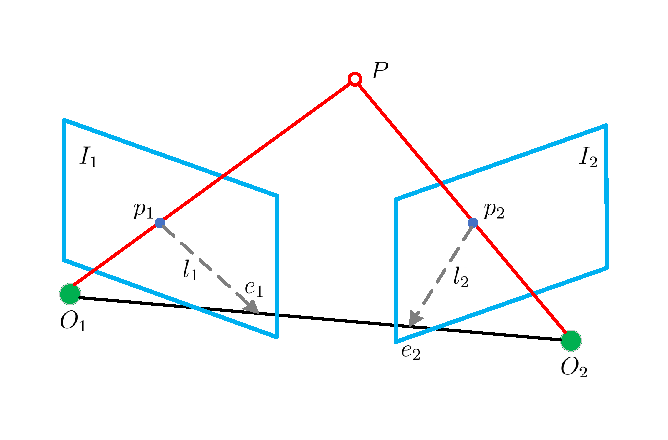
\includegraphics[width=0.25\textwidth, angle=-90]{figures/chapter3/fig3_8}
	\caption{对极几何约束示意图}\label{fig3_8}
\end{figure}

假设 $P$ 的3D空间坐标为 $\boldsymbol{P}=[X, Y, Z]^{T} $ ,根据2.1.1小节研究的针孔相机模型,可以得到 $P$ 与 $p_1,p_2 $ 的关系为:
\begin{equation}
\label{eqn:3.58}
\setlength{\abovedisplayskip}{6pt}
\setlength{\belowdisplayskip}{6pt}
\begin{aligned}
s_{1} \boldsymbol{p}_{1} &= \boldsymbol{K} \boldsymbol{P},  \\
s_{2} \boldsymbol{p}_{2} &= \boldsymbol{K}(\boldsymbol{R} \boldsymbol{P}+\boldsymbol{t})
\end{aligned}
\end{equation}
其中, $\bm{K} $ 为相机内参, $s_1,s_2 $ 为尺度因子。如果使用齐次坐标,式(\ref{eqn:3.58})可以写为:
\begin{equation}
\label{eqn:3.59}
\setlength{\abovedisplayskip}{6pt}
\setlength{\belowdisplayskip}{6pt}
\begin{aligned}
\boldsymbol{p}_{1} &= \boldsymbol{K} \boldsymbol{P},  \\
\boldsymbol{p}_{2} &= \boldsymbol{K}(\boldsymbol{R} \boldsymbol{P}+\boldsymbol{t})
\end{aligned}
\end{equation}
设 $p_1,p_2 $ 的归一化平面坐标为 $\boldsymbol{x}_{1}, \boldsymbol{x}_{2} $ ,易知:
\begin{equation}
\label{eqn:3.60}
\setlength{\abovedisplayskip}{6pt}
\setlength{\belowdisplayskip}{6pt}
\begin{aligned}
\boldsymbol{x}_{1} &=\boldsymbol{K}^{-1} \boldsymbol{p}_{1} \\
\boldsymbol{x}_{2} &=\boldsymbol{K}^{-1} \boldsymbol{p}_{2}
\end{aligned}
\end{equation}
联立式(\ref{eqn:3.59})和(\ref{eqn:3.60})可得:
\begin{equation}
\label{eqn:3.61}
\boldsymbol{x}_{2}=\boldsymbol{R} \boldsymbol{x}_{1}+\boldsymbol{t}
\end{equation}
等式(\ref{eqn:2.61})两边同时左乘 $\left[\bm{t}\right]_\times $ 可得:
\begin{equation}
\label{eqn:3.62}
\setlength{\abovedisplayskip}{6pt}
\setlength{\belowdisplayskip}{6pt}
\left[\boldsymbol{t}\right]_\times \boldsymbol{x}_{2}= \left[\boldsymbol{t}\right]_\times  \boldsymbol{R} \boldsymbol{x}_{1}
\end{equation}
等式(\ref{eqn:3.62})两边同时左乘 $\bm{x}_{2}^{T} $ 可得:
\begin{equation}
\label{eqn:3.63}
\setlength{\abovedisplayskip}{6pt}
\setlength{\belowdisplayskip}{6pt}
\boldsymbol{x}_{2}^{T} \left[\boldsymbol{t}\right]_\times \boldsymbol{x}_{2}=
\boldsymbol{x}_{2}^{T} \left[\boldsymbol{t}\right]_\times \boldsymbol{R} \boldsymbol{x}_{1}
\end{equation}
由于向量 $\left[\boldsymbol{t}\right]_\times \boldsymbol{x}_{2} $ 和 $\bm{x}_2 $ 垂直,所以等式(\ref{eqn:3.63})左侧等于0,所以:
\begin{equation}
\label{eqn:3.64}
\setlength{\abovedisplayskip}{6pt}
\setlength{\belowdisplayskip}{6pt}
\boldsymbol{x}_{2}^{T} \left[\boldsymbol{t}\right]_\times \boldsymbol{R} \boldsymbol{x}_{1} = 0
\end{equation}
联立公式(\ref{eqn:3.60})和(\ref{eqn:3.64})可得:
\begin{equation}
\label{eqn:3.65}
\setlength{\abovedisplayskip}{6pt}
\setlength{\belowdisplayskip}{6pt}
\boldsymbol{p}_{2}^{T} \boldsymbol{K}^{-T} \left[\boldsymbol{t}\right]_\times \boldsymbol{R} \boldsymbol{K}^{-1} \boldsymbol{p}_{1}=0
\end{equation}
公式(\ref{eqn:3.64})和(\ref{eqn:3.65})称为对极约束,其几何意义是 $O_{1}, P, O_{2} $ 三点共面。记
\begin{equation}
\label{eqn:3.66}
\setlength{\abovedisplayskip}{6pt}
\setlength{\belowdisplayskip}{6pt}
\begin{aligned}
\boldsymbol{E} &= \left[\boldsymbol{t}\right]_\times \boldsymbol{R} \\
\boldsymbol{F} &= \boldsymbol{K}^{-T} \left[\boldsymbol{t}\right]_\times \boldsymbol{R} \boldsymbol{K}^{-1} \\
&= \boldsymbol{K}^{-T} \boldsymbol{E} \boldsymbol{K}^{-1} 
\end{aligned}
\end{equation}
称 $\boldsymbol{F} $ 为基本矩阵,$\boldsymbol{E} $ 为本质矩阵。可见 $\boldsymbol{F} $ 和 $\boldsymbol{E} $ 之间只相差了一个相机内参 。这样以来,就可以根据匹配的关键点,通过对极约束求出 $\boldsymbol{F} $ 或者 $\boldsymbol{E} $ ,进而求出 $\boldsymbol{R}, \boldsymbol{t} $ 。

矩阵 $\left[\boldsymbol{t}\right]_\times \boldsymbol{R}  $ 有六个自由度,由对极约束(\ref{eqn:3.64})可知 $\bm{E} $ 具有尺度不确定性,所以 $\bm{E} $ 只有五个自由度。这表明,最少使用五对匹配的关键点就可以求出 $\bm{E} $ \upcite{nister2004efficient}。由于本质矩阵 $\bm{E} $ 的奇异值形式是 $[\sigma, \sigma, 0]^{T} $ \upcite{hartley2003multiple},这种非线性性质使得求解线性方程变得困难。因此,通常使用八对匹配的关键点来求解 $\bm{E} $ ,这种方法称为八点发(Eight-point-algorithm)\upcite{hartley2003multiple}\upcite{Hartley1997In}\upcite{longuet1981computer}。

假设有一对匹配好的关键点,其归一化的齐次坐标为:$\boldsymbol{x}_{1}=\left[u_{1}, v_{1}, 1\right]^{T}$ ,$\boldsymbol{x}_{2}=\left[u_{2}, v_{2}, 1\right]^{T}  $ 。由对极约束(3.64)可得,
\begin{equation}
\label{eqn:3.67}
\left(u_{1}, v_{1}, 1\right) \left( \begin{array}{ccc}{e_{1}} & {e_{2}} & {e_{3}} \\ {e_{4}} & {e_{5}} & {e_{6}} \\ {e_{7}} & {e_{8}} & {e_{9}}\end{array}\right) \left( \begin{array}{l}{u_{2}} \\ {v_{2}} \\ {1}\end{array}\right)=0
\end{equation}
中间的矩阵是本质矩阵 $\bm{E} $ 。改变 $\bm{E} $ 的形式,令 $ \boldsymbol e=\left[e_{1}, e_{2}, e_{3}, e_{4}, e_{5}, e_{6}, e_{7}, e_{8}, e_{9}\right]^{T} $ ,则式(\ref{eqn:3.67})可变形为:
\begin{equation}
\label{eqn:3.68}
\setlength{\abovedisplayskip}{6pt}
\setlength{\belowdisplayskip}{6pt}
\left[u_{1} u_{2}, u_{1} v_{2}, u_{1}, v_{1} u_{2}, v_{1} v_{2}, v_{1}, u_{2}, v_{2}, 1\right] \cdot \boldsymbol e=0
\end{equation}

对于其他七个点可以得到类似的方程,将这八个方程放在一起写成矩阵的形式,可得:
\begin{equation}
\label{eqn:3.69}
\left( \begin{array}{ccccccccc}
{u_{1}^{1} u_{2}^{1}} & {u_{1}^{1} v_{2}^{1}} & {u_{1}^{1}} & {v_{1}^{1} u_{2}^{1}} & {v_{1}^{1} v_{2}^{1}} & {v_{1}^{1}} & {u_{2}^{1}} & {v_{2}^{1}} & {1}  \\ 
{u_{1}^{2} u_{2}^{2}} & {u_{1}^{2} v_{2}^{2}} & {u_{1}^{2}} & {v_{1}^{2} u_{2}^{2}} & {v_{1}^{2} v_{2}^{2}} & {v_{1}^{2}} & {u_{2}^{2}} & {v_{2}^{2}} & {1} \\ 
{\vdots} & {\vdots} & {\vdots} & {\vdots} & {\vdots} & {\vdots} & {\vdots} & {\vdots} \\ 
{u_{1}^{8} u_{2}^{8}} & {u_{1}^{8} v_{2}^{8}} & {u_{1}^{8}} & {v_{1}^{8} u_{2}^{8}} & {v_{1}^{8} v_{2}^{8}} & {v_{1}^{8}} & {u_{2}^{8}} & {v_{2}^{8}} & {1}
\end{array}\right)
\left( \begin{array}{c}{e_{1}} \\ {e_{2}} \\ {e_{3}} \\ {e_{4}} \\ {e_{5}} \\ {e_{6}} \\ {e_{8}} \\ {e_{8}} \\ {e_{9}}\end{array}\right)
=0
\end{equation}

通过求解这个方程组就可以得到本质矩阵  $\bm{E} $ ,然后通过奇异值分解(SVD)来计算 $\boldsymbol{R}, \boldsymbol{t} $ 。假设  $\bm{E} $  的奇异值分解为:
\begin{equation}
\label{eqn:3.70}
\setlength{\abovedisplayskip}{6pt}
\setlength{\belowdisplayskip}{6pt}
\boldsymbol{E}= \boldsymbol{U} \boldsymbol{\Sigma} \boldsymbol{V}^{T}
\end{equation}
其中,$\boldsymbol{U},\boldsymbol{V} $ 是正交矩阵,$\boldsymbol{\Sigma} $ 是奇异值矩阵。由 $\bm{E} $ 的非线性性质可得 $\boldsymbol{\Sigma}=\operatorname{diag}(\sigma, \sigma, 0) $ 。在SVD分解过程中可以发现,一个本质矩阵对应两组可能的 $\boldsymbol{R}, \boldsymbol{t} $:
\begin{equation}
\label{eqn:3.71}
\begin{aligned}
\left[\boldsymbol{t}_{1}\right]_\times&= \boldsymbol{U} \boldsymbol{R}_{Z}\left(\frac{\pi}{2}\right) \boldsymbol{\Sigma} \boldsymbol{U}^{T}, \quad \boldsymbol{R}_{1}=\boldsymbol{U} \boldsymbol{R}_{Z}^{T}\left(\frac{\pi}{2}\right) \boldsymbol{V}^{T} \\
\left[\boldsymbol{t}_{2}\right]_\times &= \boldsymbol{U} \boldsymbol{R}_{Z}\left(-\frac{\pi}{2}\right) \boldsymbol{\Sigma} \boldsymbol{U}^{T}, \quad \boldsymbol{R}_{2}=\boldsymbol{U} \boldsymbol{R}_{Z}^{T}\left(-\frac{\pi}{2}\right) \boldsymbol{V}^{T} 
\end{aligned}
\end{equation}
其中,$\boldsymbol{R}_{Z}\left(\frac{\pi}{2}\right) $ 表示绕 轴旋转90°的旋转矩阵。$\bm{E} $ 的尺度不确定性导致 $\bm{E} $ 和 $-\bm{E} $ 是等价的,故对于 $-t$ 也会得到式(\ref{eqn:3.71})的结果。所以总共有四种可能的情况,如图\ref{fig3_9}所示。根据实际情况,分解出来的 $\boldsymbol{R}, \boldsymbol{t} $ 应该满足使得路标点的深度为正值,也就是说关键点对应的3D空间点 $P$ 应该和相机成像平面在同一侧,可见在图\ref{fig3_9}的4种情形中,只有第一种符合要求,从而确定该解为正确的解。
\begin{figure}[h]\setlength{\belowcaptionskip}{-12pt}
	\centering
	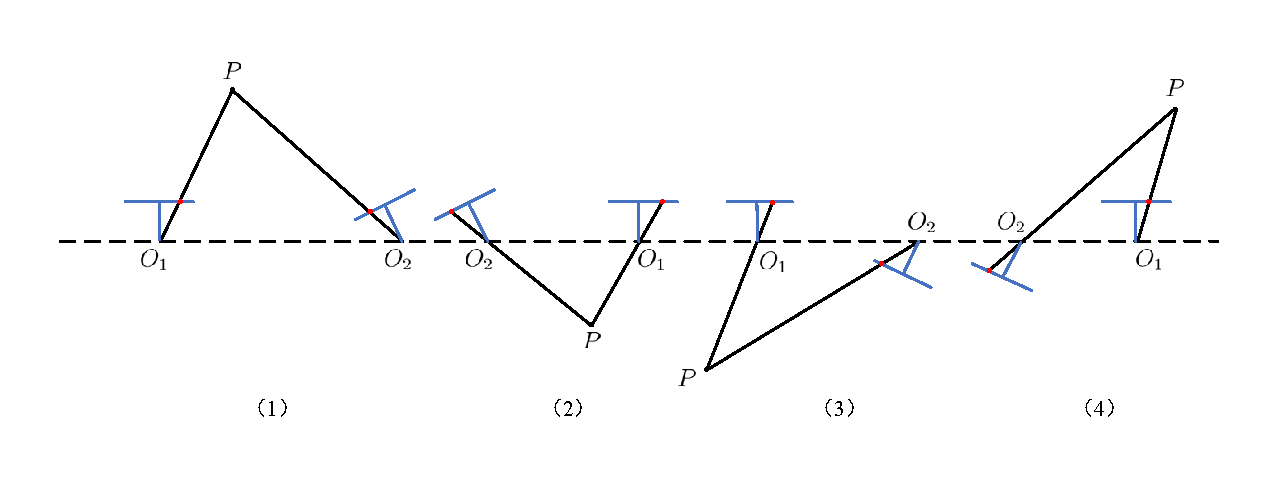
\includegraphics[width=0.3\textwidth, angle=-90]{figures/chapter3/fig3_9}
	\caption{分解本质矩阵得到的四种解}\label{fig3_9}
\end{figure}

2.三角化求路标点深度

在单目视觉SLAM中,无法直接获取路标点的深度信息,需要利用相机位姿通过三角测量(Triangulation,也称三角化)的方法来计算路标点深度。三角测量是指,在不同的方向观察目标点,通过两次观察的方向与目标点的夹角来确定目标的的距离。三角测量由高斯最先提出,在地理学和天文学中都有广泛的应用。与图\ref{fig3_8}类似,图\ref{fig3_10}展示了三角化计算路标点深度的示意图。
\begin{figure}[h]\setlength{\belowcaptionskip}{-12pt}
	\centering
	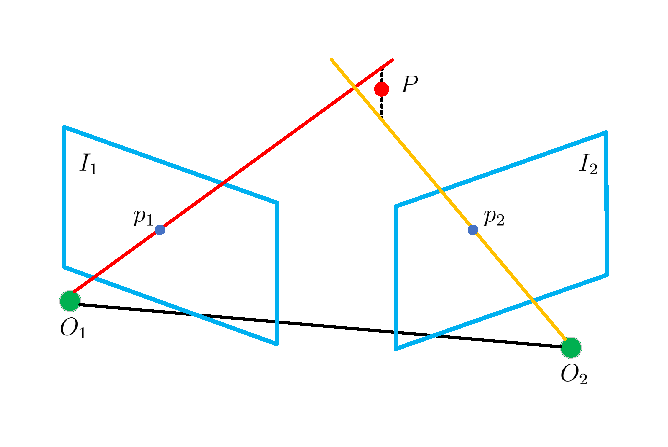
\includegraphics[width=0.25\textwidth, angle=-90]{figures/chapter3/fig3_10}
	\caption{三角化计算路标点深度}\label{fig3_10}
\end{figure}

以左边图像 $I_1 $ 为参考帧,假设右边图像  $I_2 $ 的旋转和平移为 $\boldsymbol{R}, \boldsymbol{t} $ 。理想情况下,射线 $O_1p_1 $ 和射线$O_2p_2 $ 会相交于点 $P$ ,点 $P$ 是 $p_1,p_2 $ 对应的三维空间坐标点。但是,实际情况下,由于传感器有噪声,射线 $O_1p_1 $ 和射线$O_2p_2 $通常不会严格的相交于点 $P$ ,甚至在三维空间中都不能相交。这种情况下通常利用最小二乘法来求解。

设 $\boldsymbol{x}_{1}, \boldsymbol{x}_{2} $ 是 $p_1,p_2 $ 的归一化坐标,由对极约束可得:
\begin{equation}
\label{eqn:3.72}
\setlength{\abovedisplayskip}{6pt}
\setlength{\belowdisplayskip}{6pt}
s_{1} \boldsymbol{x}_{1}=s_{2} \boldsymbol{R} \boldsymbol{x}_{2}+\boldsymbol{t}
\end{equation}
其中 $s_{1}, s_{2} $ 分别为 $p_1,p_2 $ 的深度。将等式(\ref{eqn:3.72})两边同时乘以 $\left[ \bm{x}_1 \right]_\times$ 得,
\begin{equation}
\label{eqn:3.73}
\setlength{\abovedisplayskip}{6pt}
\setlength{\belowdisplayskip}{6pt}
s_{1} \left[\boldsymbol{x}_{1}\right]_\times \boldsymbol{x}_{1}=0=s_{2} \left[\boldsymbol{x}_{1}\right]_\times \boldsymbol{R} \boldsymbol{x}_{2}+ \left[\boldsymbol{x}_{1}\right]_\times \boldsymbol{t}
\end{equation}

因为 $\boldsymbol{R}, \boldsymbol{t} $ 已知,故可以直接算出深度 $s_2 $ 。同理可得 $s_1 $ 。当然,根据刚才的分析,噪声的存在会使等式(3.73)不严格的等于0。所以需使用最小二乘法求解。

值得注意的是,由于本质矩阵 $\bm{E} $ 的尺度不确定性,计算出的路标点深度是没有尺度的,只有大小,也就是说此时得到的深度没有单位度量。在后面的联合初始化中,通过将视觉和IMU对齐来恢复出单目视觉的尺度信息。

三角测量是通过在不同的方向上观察路标点计算而得到的深度,因此相机必须要有平移,在纯旋转的情况下三角测量失效。在有平移的情况下,三角测量还存在一个矛盾的问题。这个矛盾是由像素的不确定性导致的。

如图\ref{fig3_11}所示,当相机的平移 $t$ 很小时,像素由于相机测量噪声产生的微小不确定性 $\delta \theta $,将导致计算的深度值有较大的不确定性$\delta d $ 。对比图\ref{fig3_11}的左右两图可以发现,当像素不确定性一样的情况下,较大的平移  $t$ 会产生更小的深度不确定性 $\delta d $ 。所以,在相机分辨率一样的情况下,较大的平移会使得三角测量更准确。
但是,并不是平移量越大越好,因为太大的平移量会图像特征跟踪(匹配)失败。因此就会产生一个三角化矛盾:增大平移会导致特征跟踪(匹配)失败,而减小平移又会降低三角测量的精度。
\begin{figure}[h]\setlength{\belowcaptionskip}{-12pt}
	\centering
	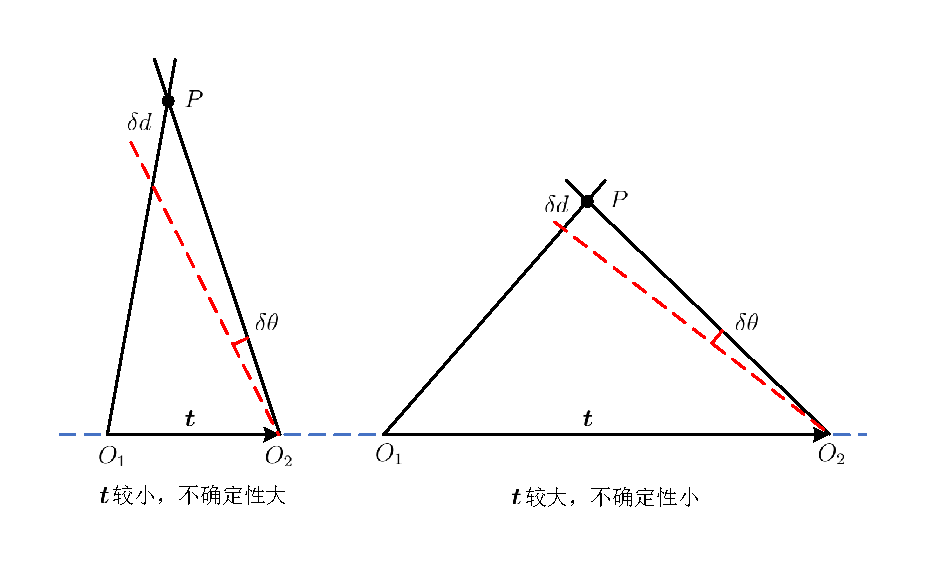
\includegraphics[width=0.35\textwidth, angle=-90]{figures/chapter3/fig3_11}
	\caption{三角测量的矛盾}\label{fig3_11}
\end{figure}

3.PnP求位姿

通过对极约束和三角测量已经可以计算出相机的姿态以及路标点的3D空间位置(没有尺度信息),那么能否根据已经计算出来的3D路标点,以及该路标点在其他图像帧中的2D投影坐标,来计算其他图像帧对应的相机姿态呢?当然可以,PnP正是求解此问题的方法,也就是说,当知道$n$个3D空间点以及他们在图像中的投影位置时,可以用PnP来求解相机的位姿。

求解PnP有很多种方法,比如使用3对点的P3P\upcite{gao2003complete},直接线性变换(Direct Linear Transform,DLT),EPnP(Efficient PnP)\upcite{lepetit2009epnp},UPnP\upcite{penate2013exhaustive}等等。下面研究DLT方法。

假设3D空间中的一点 $P$ ,用齐次坐标表示为 $\boldsymbol{P}=(X, Y, Z, 1)^{T} $ ,其在某一副图像中的投影点为 $\boldsymbol{x}_{1}$ ,用齐次坐标表示其在归一化平面上的坐标 $\boldsymbol{x}_{1}=\left(u_{1}, v_{1}, 1\right)^{T} $ 。该图像对应的相机位姿为 $\boldsymbol{R}, \boldsymbol{t} $ ,将 $\boldsymbol{R}, \boldsymbol{t} $ 放在一起构成一个增广矩阵 $\boldsymbol{T}= [ \boldsymbol{R} | \boldsymbol{t}] $ , $ \boldsymbol{T} $ 为3×4矩阵。根据3D空间点和归一化平面坐标点之间的映射关系可得,
\begin{equation}
\label{eqn:3.74}
s \left( \begin{array}{c}{u_{1}} \\ {v_{1}} \\ {1}\end{array}\right)=\left( \begin{array}{cccc}{t_{1}} & {t_{2}} & {t_{3}} & {t_{4}} \\ {t_{5}} & {t_{6}} & {t_{7}} & {t_{8}} \\ {t_{9}} & {t_{10}} & {t_{11}} & {t_{12}}\end{array}\right) \left( \begin{array}{c}{X} \\ {Y} \\ {Z} \\ {1}\end{array}\right)
\end{equation}
其中,中间得矩阵为 $ \boldsymbol{T} $ 的展开式。可以利用最后一行等式将式(\ref{eqn:3.74})中的尺度 $s$ 消去,得到两个约束等式:
\begin{equation}
\label{eqn:3.75}
\begin{aligned}
u_{1} &= \frac{t_{1} X+t_{2} Y+t_{3} Z+t_{4}}{t_{9} X+t_{10} Y+t_{11} Z+t_{12}} \\
v_{1} &= \frac{t_{5} X+t_{6} Y+t_{7} Z+t_{8}}{t_{9} X+t_{10} Y+t_{11} Z+t_{12}}
\end{aligned}
\end{equation}
令 $ \boldsymbol{T} $ 的行向量为:
\begin{equation}
\label{eqn:3.76}
\begin{aligned}
\boldsymbol{t} _{1} &= \left(t_{1}, t_{2}, t_{3}, t_{4}\right)^{T} \\
\boldsymbol{t} _{2} &= \left(t_{5}, t_{6}, t_{7}, t_{8}\right)^{T} \\
\boldsymbol{t} _{3} &= \left(t_{9}, t_{10}, t_{11}, t_{12}\right)^{T}
\end{aligned}
\end{equation}
则式(\ref{eqn:3.75})可以写为:
\begin{equation}
\label{eqn:3.77}
\begin{aligned}
\boldsymbol{t}_{1}^{T} \boldsymbol{P}-\boldsymbol{t}_{3}^{T} \boldsymbol{P} u_{1}=0 \\
\boldsymbol{t}_{2}^{T} \boldsymbol{P}-\boldsymbol{t}_{3}^{T} \boldsymbol{P} v_{1}=0
\end{aligned}
\end{equation}

可以观察到,一对3D路标点和2D关键点可以提供两个关于关于 $t$ 的线性约束项等式。那么 $N$ 对3D路标点和2D关键点可以提供 $2N$ 个约束项,写成矩阵形式为:
\begin{equation}
\label{eqn:3.78}
\left( \begin{array}{ccc}{\boldsymbol{P}_{1}^{T}} & {0} & {-u_{1} \boldsymbol{P}_{1}^{T}} \\ {0} & {\boldsymbol{P}_{1}^{T}} & {-v_{1} \boldsymbol{P}_{1}^{T}} \\ {\vdots} & {\vdots} & {\vdots} \\ {\boldsymbol{P}_{N}^{T}} & {0} & {-u_{N} \boldsymbol{P}_{N}^{T}} \\ {0} & {\boldsymbol{P}_{N}^{T}} & {-v_{N} \boldsymbol{P}_{N}^{T}}\end{array}\right) 
\left( \begin{array}{l}{\boldsymbol{t}_{1}} \\ {\boldsymbol{t}_{2}} \\ {\boldsymbol{t}_{3}}\end{array}\right)=0
\end{equation}
 $t$ 的维数为12,因此最少可以通过6对3D路标点和2D关键点就可以求解出矩阵 $ \boldsymbol{T} $ 。当匹配或跟踪的点对大于6对时,可以使用SVD方法求解。
 
 4.Bundle Adjustment
 
 BA(Bundle Adjustment)中文可译为“捆集调整”\upcite{triggs1999bundle}\upcite{granshaw1980bundle}。通过最小化重投影误差(Reprojection Error)来迭代优化求解问题。对于单目相机来说,使用PnP需要先求相机位姿,在求3D路标点位置,而BA将相机位姿和路标点位置看作优化变量,放在一起进行迭代优化。通常情况下,用BA来优化PnP估计的结果。
 
 假设有 $n$ 个3D空间点 $P$ ,在某一副图像中对应的投影坐标点为 $p$ ,第 $i$ 个3D空间点的坐标为 $\bm{P}_{i}=\left[X_{i}, Y_{i}, Z_{i}\right]^{T} $ ,对应的投影像素坐标为 $\boldsymbol{u}_{i}=\left[u_{i}, v_{i}\right]^{T} $。该图像对应的相机位姿为 $\bm{R}, \bm{t} $ ,其李代数为 $ \exp \left( \left[ \boldsymbol{\xi} \right]_\times \right) $ 。根据针孔相机模型可得:
\begin{equation}
\label{eqn:3.79}
\begin{aligned}
s_{i} \boldsymbol{u}_{i} &= \boldsymbol{K} \exp \left(  \left[\boldsymbol{\xi}\right]_\times  \right) \boldsymbol{P}_{i} \\
s_{i} \left[ \begin{array}{c}{u_{i}} \\ {v_{i}} \\ {1}\end{array}\right] &= \boldsymbol{K} \exp \left(  \left[\boldsymbol{\xi}\right]_\times \right) \left[ \begin{array}{c}{X_{i}} \\ {Y_{i}} \\ {Z_{i}} \\ {1}\end{array}\right]
\end{aligned}
\end{equation}
其中,$s_i $ 是尺度,$\bm{K} $ 是相机内参。然而,实际情况中相机是有噪声的,噪声使得等式(\ref{eqn:3.79})不相等,有一个误差。将每个观测点噪声带来的误差相加构成一个代价函数,建模为最小二乘问题,通过最小化代价函数来寻找最优的 $\bm{P}_i$ 和 $ \left[\boldsymbol{\xi}\right]_\times  $ :
\begin{equation}
\label{eqn:3.80}
\boldsymbol{e} =\arg \min _{\boldsymbol{\xi}} \frac{1}{2} \sum_{i=1}^{n}\left\|\boldsymbol{u}_{i}-\frac{1}{s_{i}} \boldsymbol{K} \exp \left(  \left[\boldsymbol{\xi}\right]_\times  \right) \boldsymbol{P}_{i}\right\|_{2}^{2}
\end{equation}

对于最小二乘问题,通常使用高斯-牛顿法或者LM方法求解。在使用G-N或者L-M方法的时候,需要知道代价函数关于误差项的导数,也就是雅可比矩阵,这里不再详细推导,直接给出代价函数 $\boldsymbol{e} $ 关于相机位姿 $\boldsymbol{\xi} $ 和3D空间点 $P$ 的的雅可比矩阵:
\begin{equation}
\label{eqn:3.81}
\frac{\partial \bm{e}}{\partial \delta \bm{\xi}} = 
-\left[ \begin{array}{cccccc}
{\frac{f_{x}}{Z^{\prime}}} & {0} & {-\frac{f_{x} X^{\prime}}{Z^{\prime 2}}} &
{-\frac{f_{x} X^{\prime} Y^{\prime}}{Z^{\prime 2}}} & {f_{x}+\frac{f_{x} X^{2}}{Z^{\prime 2}}} & {-\frac{f_{x} Y^{\prime}}{Z^{\prime}}}  \\ 
{0} & {\frac{f_{y}}{Z^{\prime}}} & {-\frac{f_{y} Y^{\prime}}{Z^{\prime 2}}} &
{-f_{y}-\frac{f_{y} Y^{\prime 2}}{Z^{\prime 2}}} & {\frac{f_{y} X^{\prime} Y^{\prime}}{Z^{\prime 2}}} & {\frac{f_{y} X^{\prime}}{Z^{\prime}}} 
\end{array}\right]
\end{equation}
\begin{equation}
\label{eqn:3.82}
\frac{\partial \bm{e}}{\partial \boldsymbol{P}}=-\left[ \begin{array}{ccc}{\frac{f_{x}}{Z^{\prime}}} & {0} & {-\frac{f_{x} X^{\prime}}{Z^{\prime 2}}} \\ {0} & {\frac{f_{y}}{Z^{\prime}}} & {-\frac{f_{y} Y^{\prime}}{Z^{\prime 2}}}\end{array}\right] \boldsymbol{R}
\end{equation}
\subsection{纯视觉初始化}
为了减少计算量,初始化在一个滑动窗口内进行。首先检查窗口内当前的图像帧与其他帧的关键点对应关系,找到与当前帧匹配关键点数量最多的关键帧作为参考帧。然后使用对极几何求解基础矩阵,从而计算出当前帧与参考帧帧之间的变换矩阵。然后用SFM(Structure-From-Motion)\upcite{ullman1979interpretation}计算处滑窗内的所有关键帧的位姿以及路标点的3D空间坐标,SFM具体步骤包括:

(1)通过三角化得到当前帧和参考帧的路标点;

(2)对于当前帧和参考帧之间的所有帧用PnP算法求解其位姿;

(3)通过三角化得到当前帧和参考帧之间的所有帧的路标点;

(4)对于当前帧和第一帧之间的所有帧用PnP算法求解其位姿;

(5)通过三角化得到当前帧和第一帧之间的所有帧的路标点;

(6)对于其他没有被三角化的关键点,对其三角化得到剩余的路标点;

(7)通过BA对滑动窗口内的所有关键帧位姿进行优化。

在完成了SFM后,已经可以估计出滑动窗口内所有关键帧的位姿,然而,视觉初始化可能不是一次就能成功,这个时候,关键帧的总数可能会超过窗口大小,还需要再次使用PnP算法估计出那些不被包括在窗口内的关键帧的位姿。

至此,纯视觉初始化就完成了。值得注意的是,在纯视觉初始化的时候,将第一帧图像$ {(\cdot)}^{c_0} $ 作为参考帧,因此需要将位姿从第一帧图像坐标系转换到IMU坐标系,方法如下:
\begin{equation}
\label{eqn:3.83}
\begin{split}
\mathbf{q}_{b_k}^{c_0}&=\mathbf{q}_{c_k}^{c_0}\otimes(\mathbf{q_c^b})^{-1} \\
s\bar{\mathbf{p}}_{b_k}^{c_0}&=s\bar{\mathbf{p}}_{c_k}^{c_0}-\mathbf{R}_{b_k}^{c_0}\mathbf{p}_c^b,
\end{split}
\end{equation}
其中,$ \mathbf{p}_c^b,\mathbf{q}_c^b $ 是外参(Visual到IMU)。
\subsection{视觉/惯性联合初始化}
如图\ref{fig3_12}所示,视觉/惯性联合初始化是将IMU预积分的值和出视觉初始化的值进行对齐,从而计算出绝对尺度 $s $ 、陀螺仪bias、重力矢量 $\mathbf{g} $ 和速度 $\mathbf{v}$ 。注意,不计算加速度计的bias,因为重力加速度的值要远远大于加速度计的bias,这导致加速度计的bias很难被观测到\upcite{mur2017visual},因此忽略加速度计bias的影响,只计算陀螺仪的bias。
\begin{figure}[h]\setlength{\belowcaptionskip}{-12pt}
	\centering
	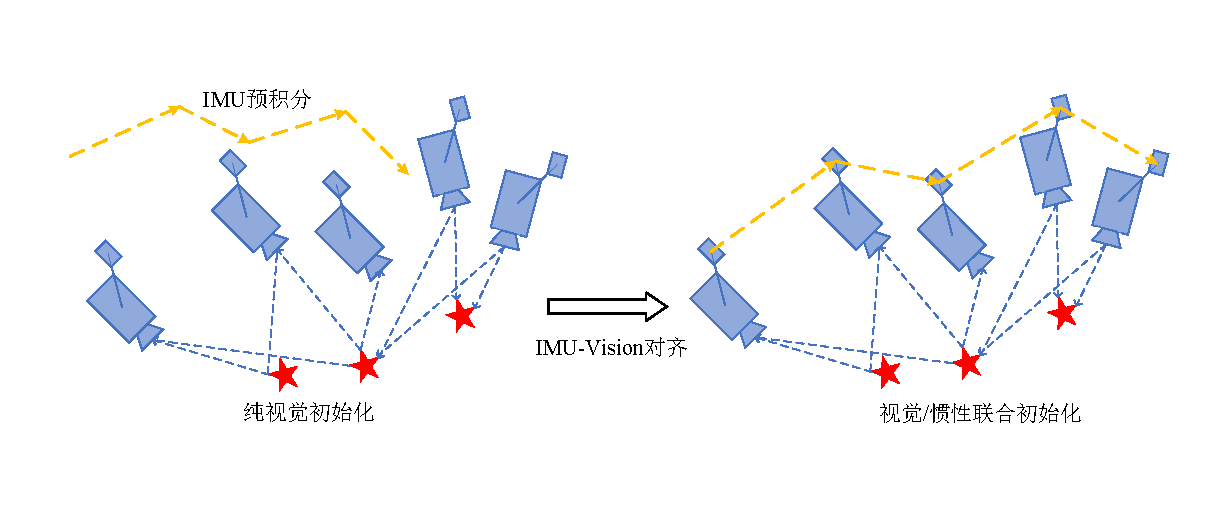
\includegraphics[width=0.3\textwidth, angle=-90]{figures/chapter3/fig3_12}
	\caption{视觉/惯性联合初始化示意图}\label{fig3_12}
\end{figure}

(1)矫正陀螺仪bias

考虑滑动窗口内连续两帧图像 $ b_k $ 和 $b_{k+1}$ ,从纯视觉初始化中得到的两帧之间的旋转 $ {\mathbf{q}_{b_{k+1}}^{c_0}}^{-1} \mathbf{q}_{b_k}^{c_0} $  应该和IMU预积分得到旋转 $ \bm{\gamma}_{b_{k+1}}^{b_k} $ 相等。通过式(3.18) 线性化IMU预积分项,并定义代价函数:
\begin{equation}
\label{eqn:3.84}
\underset{\delta b_w}{\text{min}}\sum_{k\in \mathcal{B} }\left\|{\mathbf{q}_{b_{k+1}}^{c_0}}^{-1}\otimes\mathbf{q}_{b_k}^{c_0}\otimes\bm{\gamma}_{b_{k+1}}^{b_k}\right\|^2 
\end{equation}
其中,$\mathcal{B} $ 代表窗口中的所有帧,
\begin{equation}
\label{eqn:3.85}
\bm{\gamma}_{b_{k+1}}^{b_k}\approx\hat{\bm{\gamma}}_{b_{k+1}}^{b_k}\otimes\begin{bmatrix}
1 \\ \frac{1}{2}\mathbf{J}_{b_w}^\gamma\delta\mathbf{b}_w
\end{bmatrix}
\end{equation}
代价函数(\ref{eqn:3.84})的最小值为单位四元数,所以可以将式(\ref{eqn:3.84})写为:
\begin{equation}
\label{eqn:3.86}
{ \mathbf{ q}_{b_{k+1}}^{c_{0}}}^{-1} \otimes \mathbf{q}_{b_{k}}^{c_{0}} \otimes \bm{\gamma}_{b_{k+1}}^{b_{k}}=\left[ \begin{array}{l}{\mathbf{1}} \\ {0}\end{array}\right]
\end{equation}
将式(\ref{eqn:3.85})代入式(\ref{eqn:3.86})得,
\begin{equation}
\label{eqn:3.87}
\begin{aligned}
\hat{\bm{\gamma}}_{b_{k+1}}^{b_{k}} \otimes\left[\frac{1}{2} \mathbf{J}_{b_{\omega}}^{\gamma} \delta \mathbf{b}_{\omega}\right]
&= \mathbf{q}_{b_{k}}^{c_{0}-1} \otimes \mathbf{q}_{b_{k+1}}^{c_{0}} \otimes \left[ \begin{array}{l}{\mathbf{1}} \\ {0}\end{array}\right] \\
\Longrightarrow \quad \quad \left[\frac{1}{2} \mathbf{J}_{b_{\omega}}^{\gamma} \delta \mathbf{b}_{\omega}\right]
&= \hat{\bm{\gamma}}_{b_{k+1}}^{b_{k}-1} \otimes \mathbf{q}_{b_{k}}^{c_{0}-1} \otimes \mathbf{q}_{b_{k+1}}^{c_{0}} \otimes \left[ \begin{array}{l}{\mathbf{1}} \\ {0}\end{array}\right] \\
\Longrightarrow \quad \quad \quad \quad  \mathbf{J}_{b_{\omega}}^{\gamma} \delta \mathbf{ b}_{\omega} 
&=2 \mathbf{Im}\left( (\hat{\bm{\gamma}}^{b_{k}}_{b_{k+1}})^{-1} \otimes \mathbf{q}_{b_{k}}^{c_{0}-1} \otimes \mathbf{q}_{b_{k+1}}^{c_{0}}\right)
\end{aligned}
\end{equation}
其中 $\mathbf{Im} $ 表示虚部。将式(3.87)两边同时乘以 ${\mathbf{J}_{b_{\omega}}^{\gamma}}^{T}$ ,使等式左边变为正定矩阵,
\begin{equation}
\label{eqn:3.88}
{\mathbf{J}_{b_{\omega}}^{\gamma}}^{T}
\mathbf{J}_{b_{\omega}}^{\gamma} \delta \mathbf{b}_{\omega} = 
2 {\mathbf{J}_{b_{\omega}}^{\gamma}}^{T} \mathbf{Im}\left( (\hat{\bm{\gamma}}_{b_{k+1}}^{b_{k}})^{-1} \otimes \mathbf{q}_{b_{k}}^{c_{0}-1} \otimes \mathbf{q}_{b_{k+1}}^{c_{0}}\right)
\end{equation}

这样就可以直接通过Cholesky分解法得到陀螺仪的bias。然后再用计算出的陀螺仪bias再次重新积分IMU。

(2)速度、重力矢量和尺度因子初始化

将速度、重力和尺度因子放在一起作为优化变量,
\begin{equation}
\label{eqn:3.89}
\setlength{\abovedisplayskip}{6pt}
\setlength{\belowdisplayskip}{6pt}
\mathcal{X}_I=[\mathbf{v}_{b_0}^{b_0},\mathbf{v}_{b_1}^{b_1},\cdots\mathbf{v}_{b_n}^{b_n},\mathbf{g}^{c_0},s]
\end{equation}
其中,当取第 $k$ 帧图像时,$\mathbf{v}_{b_k}^{b_k} $ 是IMU坐标系下的速度,$ \mathbf{g}^{c_0} $ 是第0帧图像对应得相机坐标系下的重力向量,$s $ 是尺度因子。

考虑窗口中连续的两帧图像 $b_{k} $ 和 $b_{k+1} $ ,那么式(\ref{eqn:3.16})可以写成:
\begin{equation}
\label{eqn:3.90}
\begin{split}
\bm{\alpha}_{b_{k+1}}^{b_k}&=  
\mathbf{R}_{c_0}^{b_k}(s(\bar{\mathbf{p}}_{b_{k+1}}^{c_0}-\bar{\mathbf{p}}_{b_k}^{c_0})+\frac{1}{2}\mathbf{g}^{c0}\Delta t_k^2-\mathbf{R}_{b_k}^{c_0}\mathbf{v}_{b_k}^{b_k}\Delta t_k) \\
\bm{\beta}_{b_{k+1}}^{b_k}&=
\mathbf{R}_{c_0}^{b_k}(\mathbf{R}_{b_{k+1}}^{c_0}\mathbf{v}_{b_{k+1}}^{b_{k+1}}+\mathbf{g}^{c0}\Delta t_k-\mathbf{R}_{b_k}^{c_0}\mathbf{v}_{b_k}^{b_k}).
\end{split}
\end{equation}

定义残差项为  $b_{k} $ 和 $b_{k+1} $ 帧图像间的IMU预积分量 $\hat{\bm{\alpha}}_{b_{k+1}}^{b_k},\hat{\bm{\beta}}_{b_{k+1}}^{b_k} $与预测值 $\bm{\alpha}_{b_{k+1}}^{b_k},\bm{\beta}_{b_{k+1}}^{b_k} $之间的误差,
\begin{equation}
\label{eqn:3.91}
\begin{aligned}
\mathbf{r}\left(\hat{\mathbf{Z}}_{b_{k+1}}^{b_{k}}, \mathcal{X}_{I}\right)
&= 
\left[ \begin{array}{c}
{\delta \bm{\alpha}_{b_{k+1}}^{b_{k}}} \\ {\delta \bm{\beta}_{b_{k+1}}^{b_{k}}}
\end{array}\right]  \\ 
&=
\left[ \begin{array}{c}
\hat{\bm{\alpha}}_{b_{k+1}}^{b_{k}}  -  
	\mathbf{R}_{c_0}^{b_k}(s(\bar{\mathbf{p}}_{b_{k+1}}^{c_0}-\bar{\mathbf{p}}_{b_k}^{c_0})+\frac{1}{2}\mathbf{g}^{c0}\Delta t_k^2-\mathbf{R}_{b_k}^{c_0}\mathbf{v}_{b_k}^{b_k}\Delta t_k) \\ 
	\hat{\bm{\beta}}_{b_{k+1}}^{b_{k}}-
		\mathbf{R}_{c_0}^{b_k}(\mathbf{R}_{b_{k+1}}^{c_0}\mathbf{v}_{b_{k+1}}^{b_{k+1}}+\mathbf{g}^{c0}\Delta t_k-\mathbf{R}_{b_k}^{c_0}\mathbf{v}_{b_k}^{b_k})
		\end{array}\right]
		\end{aligned}
\end{equation}
将式(\ref{eqn:3.83})代入式(\ref{eqn:3.91})中的$\delta \hat{\bm{\alpha}}_{b_{k+1}}^{b_{k}} $并写成 $\mathbf{H} \mathbf{x}=\mathbf{b} $ 的形式,
\begin{equation}
\label{eqn:3.92}
\mathbf{ R}_{c_{0}}^{b_{k}}(\overline{\mathbf{ p}}_{c_{k+1}}^{c_{0}}-\overline{\mathbf{ p}}_{c_{k}}^{c_{0}})_{S}-\Delta t_{k} \mathbf{ v}_{b_{k}}^{b_{k}}
+\frac{1}{2} \mathbf{ R}_{c_{0}}^{b_{k}} \Delta t_{k}^{2} \mathbf{ g}^{c_{0}}
=\bm{\alpha}_{b_{k+1}}^{b_{k}}-\mathbf{ p}_{c}^{b_{k}} + \mathbf{R}_{c_0}^{b_k}\mathbf{ R}_{b_{k+1}}^{c_{0}} \mathbf{ p}_{c}^{b}
\end{equation}
写成矩阵形式,
\begin{equation}
\label{eqn:3.93}
\begin{aligned}
& \left[\begin{array}{cccc}
- \mathbf{I} \Delta t_{k} & 0 & \frac{1}{2} \mathbf{R}_{c_{0}}^{b_{k}} \Delta t_{k}^{2} & \mathbf{R}_{c_{0}}^{b_{k}}(\overline{\mathbf{p}}_{c_{k+1}}^{c_{0}}-\overline{\mathbf{p}}_{c_{k}}^{c_{0}}) \\
\end{array}\right]
\left[ \begin{array}{c}{\mathbf{v}_{b_{k}}^{b_{k}}} \\ {\mathbf{v}_{b_{k+1}}^{b_{k+1}}} \\ {\mathbf{g}^{c_{0}}} \\ {S} \end{array}\right] \\
&=
\bm{\alpha}_{b_{k+1}}^{b_{k}}-\mathbf{p}_{c_{0}}^{b_{k}} + \mathbf{R}_{c_0}^{b_k}\mathbf{R}_{b_{k+1}}^{c_{0}} \mathbf{p}_{c}^{b}
\end{aligned}
\end{equation}
同理,将 $\delta \hat{\bm{\beta}}_{b_{k+1}}^{b_{k}} $ 也可以写成类似式(\ref{eqn:3.93})的形式,并与式(\ref{eqn:3.93})合并写成如下矩阵形式:
\begin{equation}
\label{eqn:3.94}
\begin{aligned}
& \left[ \begin{array}{cccc}
- \mathbf{I} \Delta t_{k} & 0 & \frac{1}{2} \mathbf{R}_{c_{0}}^{b_{k}} \Delta t_{k}^{2} & \mathbf{R}_{c_{0}}^{b_{k}}(\overline{\mathbf{p}}_{c_{k+1}}^{c_{0}}-\overline{\mathbf{p}}_{c_{k}}^{c_{0}}) \\
{- \mathbf{ I}} & {\mathbf{R}_{c_{0}}^{b_{k}} \mathbf{R}_{b_{k+1}}^{c_{0}}} & {\mathbf{R}_{c_{0}}^{b_{k}} \Delta t_{k}} & {0}
\end{array}\right] 
\left[ \begin{array}{c}
{\mathbf{v}_{b_{k}}^{b_{k}}} \\ {\mathbf{v}_{b_{k+1}}^{b_{k+1}}} \\ {\mathbf{g}^{c_{0}}} \\ s
\end{array}\right] \\
&=\left[ \begin{array}{c}
\bm{\alpha}_{b_{k+1}}^{b_{k}}-\mathbf{p}_{c_{0}}^{b_{k}} + \mathbf{R}^{b_k}_{c_0}\mathbf{R}_{b_{k+1}}^{c_{0}} \mathbf{p}_{c}^{b} \\
{\bm{\beta}_{b_{k+1}}^{b_{k}}}
\end{array}\right]
\end{aligned}
\end{equation}
式(\ref{eqn:3.94})通过Cholesky分解可以解出 $\mathcal{X}_I $ 。

(3)重力矢量修正

由于噪声等原因,在上一步求出来的重力 $\mathbf{g}^{c_0} $ 是有误差的。通常情况下,重力大小是已知的,$g \approx 9.81 \mathrm{m} / \mathrm{s}^{2} $ 。因此,可以根据这个先验信息来修正上一步估计出来的 $\mathbf{g}^{c_0} $ 。
\begin{figure}[h]\setlength{\belowcaptionskip}{-12pt}
	\centering
	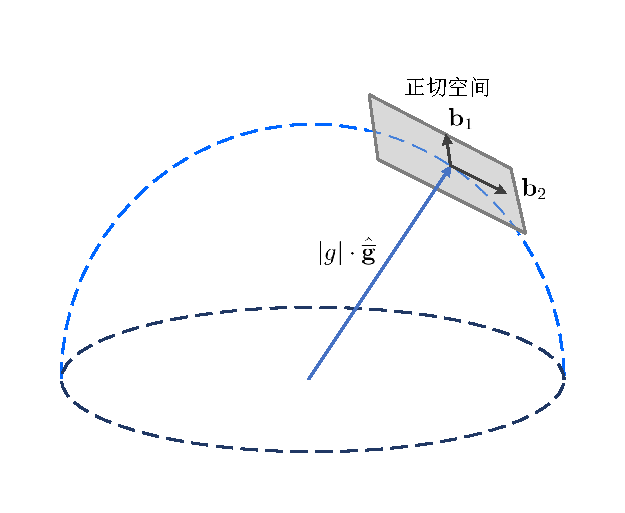
\includegraphics[width=0.25\textwidth, angle=-90]{figures/chapter3/fig3_13}
	\caption{两自由度重力矢量参数化示意图}\label{fig3_13}
\end{figure}

因为重力的大小已知,所以重力的自由度由3个变为2个。如图\ref{fig3_13},对重力重新参数化为:
\begin{equation}
\label{eqn:3.95}
\hat{\mathbf{g}} = g \cdot \overline{\hat{\mathbf{g}}} +w_{1} \mathbf{b}_{1}+w_{2} \mathbf{b}_{2}
\end{equation}
其中,$\overline{\hat{\mathbf{g}}} $ 为上一步估计出来的重力的方向向量,$\mathbf{b}_1, \mathbf{b}_2 $ 是垂直于 $\overline{\hat{\mathbf{g}}} $ 的两个正交基。

将式(3.95)代入式(3.94)可得,
\begin{equation}
\label{eqn:3.96}
\begin{aligned}
& \left[ \begin{array}{cccc}
- \mathbf{I} \Delta t_{k} & 0 & \frac{1}{2} \mathbf{R}_{c_{0}}^{b_{k}} \Delta t_{k}^{2} \mathbf{b} & \mathbf{R}_{c_{0}}^{b_{k}}(\overline{\mathbf{p}}_{c_{k+1}}^{c_{0}}-\overline{\mathbf{p}}_{c_{k}}^{c_{0}}) \\
{- \mathbf{ I}} & {\mathbf{R}_{c_{0}}^{b_{k}} \mathbf{R}_{b_{k+1}}^{c_{0}}} & {\mathbf{R}_{c_{0}}^{b_{k}} \Delta t_{k}} \mathbf{b}  & {0}
\end{array}\right] 
\left[ \begin{array}{c}
{\mathbf{v}_{b_{k}}^{b_{k}}} \\ {\mathbf{v}_{b_{k+1}}^{b_{k+1}}} \\ \bm{\omega} \\s
\end{array}\right] \\
&=\left[ \begin{array}{c}
\bm{\alpha}_{b_{k+1}}^{b_{k}}-\mathbf{p}_{c_{0}}^{b_{k}} + \mathbf{R}^{b_k}_{c_0}\mathbf{R}_{b_{k+1}}^{c_{0}} \mathbf{p}_{c}^{b} -\frac{1}{2} \mathbf{R}_{c_{0}}^{b_{k}} \Delta t_{k}^{2} g \cdot \overline{\hat{\mathrm{g}}} \\
{\bm{\beta}_{b_{k+1}}^{b_{k}}} - \mathbf{R}_{c_{0}}^{b_{k}} \Delta t_{k} g\cdot \overline{\hat{\mathrm{g}}} 
\end{array}\right]
\end{aligned}
\end{equation}
其中,$\bm{\omega} =\left[\omega_{1}, \omega_{2}\right]^{T} $ ,$\mathbf{b} =\left[b_{1}, b_{2}\right]^{T} $ 。通过求解式(\ref{eqn:3.96}),可以得到 $\bm{\omega} $ ,从而可以得到修正后的 $\mathbf{g}^{c_{0}} $。通过 $\mathbf{g}^{c_{0}} $ 和世界坐标系的 $Z$ 轴方向,可以得到第一帧图像坐标系到世界坐标系的旋转 $\mathbf{q}_{C_{0}}^{w} $ ,从而可以将所有的状态变量变换到世界坐标系下。至此,初始化完成。

(4)初始航向修正

在联合初始化完成之后,使用磁力计测量的航向角对初始化过程中估计出的每一个关键帧的航向角进行修正,从而得到无偏的初始航向。
\section{本章小结}
本章对系统的前端和初始化算法进行了详细的阐述。其中,前端部分详细研究了特征的提取、跟踪和异常点剔除算法,并对IMU预积分理论的相关公式进行了详细的推导。系统初始化部分详细研究了visual初始化算法,以及Visual-IMU对齐方法。系统的前端和初始化在整个系统中占了很大的比重,前端和初始化的好坏影响后端非线性优化的精度,从而影响整个系统的定位精度。因此,一个良好的前端和初始化是实现系统高精度定位的基础。